% =====================================================================================
% Tesis de licenciatura — Javier Orcazas — ITAM, Ciencia de Datos
%
% Estructura: este archivo solo arma el documento; el contenido vive en front/ y
% sections/. Para compilar:  pdflatex final_work && pdflatex final_work  (dos pasadas,
% la segunda resuelve índices y referencias cruzadas).
%
% NOTA DE FORMATO: la portada y la declaración de derechos siguen el formato habitual
% del ITAM, pero deben confirmarse con el asesor y con Dirección Escolar antes de
% imprimir. Los datos por confirmar están marcados con TODO en front/portada.tex.
% =====================================================================================
\documentclass[12pt,letterpaper,twoside,openright]{report}

\usepackage[utf8]{inputenc}
\usepackage[T1]{fontenc}
\usepackage[left=3cm,right=2.5cm,top=2.5cm,bottom=2.5cm]{geometry}
\usepackage{amsmath,amssymb}
\usepackage{graphicx}
\usepackage{booktabs}
\usepackage{longtable}
\usepackage{array}
\usepackage{float}
\usepackage{url}
\usepackage[round,authoryear]{natbib}
\usepackage[hidelinks]{hyperref}

\graphicspath{{images/}}

% --- Nombres en español (sin babel: no está instalado en este TeX y se prefiere que el
% --- documento compile sin dependencias adicionales). ---------------------------------
\renewcommand{\chaptername}{Capítulo}
\renewcommand{\appendixname}{Apéndice}
\renewcommand{\contentsname}{Índice general}
\renewcommand{\listfigurename}{Índice de figuras}
\renewcommand{\listtablename}{Índice de tablas}
\renewcommand{\figurename}{Figura}
\renewcommand{\tablename}{Tabla}
\renewcommand{\bibname}{Referencias}
\renewcommand{\refname}{Referencias}
\renewcommand{\abstractname}{Resumen}

% --- Macros del dominio ---------------------------------------------------------------
\newcommand{\ue}{unidad económica}
\newcommand{\UEs}{unidades económicas}
\newcommand{\horizonte}{h}

\linespread{1.25}

% --- Flotantes: permitir más figuras/tablas por página y menos páginas en blanco. -----
\renewcommand{\topfraction}{0.9}
\renewcommand{\bottomfraction}{0.85}
\renewcommand{\textfraction}{0.1}
\renewcommand{\floatpagefraction}{0.8}
\setcounter{topnumber}{3}
\setcounter{bottomnumber}{2}
\setcounter{totalnumber}{5}
\setlength{\tabcolsep}{5pt}
\renewcommand{\arraystretch}{1.1}

\begin{document}

\pagenumbering{roman}
% =====================================================================================
% PORTADA — CHECKLIST DE LO QUE FALTA LLENAR (todo lo demás ya está resuelto)
%
%   [ ] 1. Nombre y grado del asesor            -> \asesor{...} abajo
%   [ ] 2. Formato oficial vigente              -> confirmar con Dirección Escolar:
%              tipografía, orden de los elementos y si se requiere hoja de firmas aparte
%   [ ] 3. Texto de la declaración de derechos  -> front/declaracion.tex (confirmar con la
%              Biblioteca Raúl Bailléres Jr. que la redacción siga vigente)
%   [ ] 4. Agradecimientos                      -> front/agradecimientos.tex
%
% TÍTULO: decidido el 2026-08-31 — se mantiene el título nuevo, que refleja el alcance real
% (21 unidades económicas de Baja California y pronóstico probabilístico). Si el registrado
% ante Dirección Escolar es el anterior ("Predicción del volumen de pesca de langosta en San
% Quintín, Baja California"), hay que tramitar el cambio.
% =====================================================================================
\thispagestyle{empty}
\begin{center}

\vspace*{1.5cm}
{\large INSTITUTO TECNOLÓGICO AUTÓNOMO DE MÉXICO}

\vspace{2.5cm}
{\LARGE\bfseries Pronóstico calibrado del volumen de captura de langosta roja en Baja California:\\[0.3cm]
olas de calor marinas, modelos globales multi-especie e intervalos conformalizados}

\vspace{2.5cm}
{\large T\,E\,S\,I\,S}

\vspace{0.6cm}
{\large Que para obtener el título de}

\vspace{0.4cm}
{\large\bfseries LICENCIADO EN CIENCIA DE DATOS}

\vspace{0.6cm}
{\large Presenta}

\vspace{0.4cm}
{\large\bfseries JAVIER ORCAZAS}

\vspace{2.0cm}
\providecommand{\asesor}{\underline{\hspace{6cm}}\\[0.2cm]{\small\itshape pendiente: nombre y grado del asesor}}
{\large Asesor: \asesor}

\vfill
{\large CIUDAD DE MÉXICO \hfill 2026}

\end{center}
\cleardoublepage

% Declaración de derechos. TODO(Javier): verificar el texto vigente con la Biblioteca
% Raúl Bailléres Jr.; el que sigue es la formulación habitual del ITAM.
\thispagestyle{empty}
\vspace*{4cm}
\noindent
``Con fundamento en los artículos 21 y 27 de la Ley Federal del Derecho de Autor y como
titular de los derechos moral y patrimoniales de la obra titulada \emph{Pronóstico
calibrado del volumen de captura de langosta roja en Baja California: olas de calor
marinas, modelos globales multi-especie e intervalos conformalizados}, otorgo de manera
gratuita y permanente al Instituto Tecnológico Autónomo de México y a la Biblioteca Raúl
Bailléres Jr. autorización para que fijen la obra en cualquier medio, incluido el
electrónico, y la divulguen entre sus usuarios, profesores, estudiantes o terceras
personas, sin que pueda percibir por tal divulgación una contraprestación.''

\vspace{3cm}
\begin{center}
JAVIER ORCAZAS

\vspace{2cm}
\underline{\hspace{7cm}}\\
Fecha

\vspace{2cm}
\underline{\hspace{7cm}}\\
Firma
\end{center}
\cleardoublepage

% TODO(Javier): este texto es un marcador de posición; sustitúyelo por el propio.
\chapter*{Agradecimientos}
\addcontentsline{toc}{chapter}{Agradecimientos}

A Comunidad y Biodiversidad, A.C. (COBI), por abrir los datos de arribos que hacen posible
este trabajo y por el contexto pesquero que ningún conjunto de datos contiene; y a las
cooperativas de San Quintín y de la costa del Pacífico de Baja California, que son quienes
generan esos registros día con día.

TODO: agradecimientos personales y al asesor.
\cleardoublepage

\chapter*{Resumen}
\addcontentsline{toc}{chapter}{Resumen}

Las cooperativas pesqueras de Baja California necesitan anticipar el volumen de captura de
la siguiente temporada para dimensionar insumos, tripulación y compromisos de venta. Esta
tesis construye esa herramienta para la langosta roja (\emph{Panulirus interruptus}) y la
extiende a abulón y erizo, a partir de los arribos pesqueros registrados por Comunidad y
Biodiversidad, A.C.\ (COBI) y por CONAPESCA, y de variables oceanográficas satelitales
(temperatura superficial del mar y color del océano) del servicio Copernicus Marine.

El trabajo parte de una comparación de modelos de pronóstico ---ARIMA, Prophet, XGBoost,
LGBM, LSTM y su ensamble--- sobre una sola serie (langosta en San Quintín), y muestra que
ninguno explicaba la caída atípica de la temporada 2021-2022. La tesis identifica el
mecanismo faltante: las olas de calor marinas. Se implementa un índice de olas de calor
según la metodología de Hobday et al.\ (2016), que reproduce el evento ``Blob'' de 2014-2016
y el régimen cálido de 2019-2021, y se incorpora como covariable.

Sobre esa base se desarrollan tres aportaciones. Primero, un \textbf{modelo global} que
agrupa las series de especie por \ue{} del conjunto (de 28 a 33 con datos suficientes, según
el corte), con la variable objetivo en escala logarítmica, que
gana o empata contra los modelos específicos en cuatro de cinco series y rescata a las de
menor escala. Segundo, un \textbf{pronóstico probabilístico} mediante regresión cuantílica
conformalizada, que entrega intervalos con cobertura empírica cercana a la nominal y estable
incluso durante olas de calor: para una cooperativa, un rango calibrado es más accionable y
más honesto que un número puntual. Tercero, una \textbf{prueba directa de la hipótesis de
fondo} ---que el factor limitante es el volumen de datos y no la sofisticación del
modelo---: al pasar de 2 a 21 series de langosta y desbloquear las temporadas 2022-2026, la
calibración de la serie insignia se vuelve estable e invariante a la composición del pool,
mientras que ni la selección de variables por SHAP, ni la optimización bayesiana, ni un
Temporal Fusion Transformer lo consiguen. El resultado se materializa en una aplicación de
inferencia que sirve el intervalo calibrado por especie y \ue{}.

\vspace{0.5cm}
\noindent\textbf{Palabras clave:} pronóstico de series de tiempo, pesquerías, langosta roja,
Baja California, olas de calor marinas, predicción conformal, modelos globales,
interpretabilidad.

\cleardoublepage

\chapter*{Abstract}
\addcontentsline{toc}{chapter}{Abstract}

Small-scale fishing cooperatives in Baja California need to anticipate next season's catch
volume in order to plan inputs, crew and sales commitments. This thesis builds that tool for
red spiny lobster (\emph{Panulirus interruptus}), extending it to abalone and sea urchin,
using landings recorded by Comunidad y Biodiversidad, A.C.\ (COBI) and CONAPESCA together
with satellite oceanographic covariates (sea surface temperature and ocean colour) from
Copernicus Marine.

Starting from a comparison of forecasting models ---ARIMA, Prophet, XGBoost, LGBM, LSTM and
their ensemble--- on a single series, we show that none of them explained the anomalous
2021-2022 season. We identify the missing mechanism as marine heatwaves, implement the
Hobday et al.\ (2016) index ---which recovers the 2014-2016 ``Blob'' and the 2019-2021 warm
regime--- and add it as a covariate.

Three contributions follow. A \textbf{global model} pooling the dataset's species-by-cooperative series (28--33 with
enough data, depending on the cut) with a log-scaled target matches or beats series-specific models in four of five series and
rescues the small-scale ones. A \textbf{probabilistic forecast} based on conformalized
quantile regression yields intervals whose empirical coverage stays close to nominal even
during marine heatwaves; for a cooperative, a calibrated range is more actionable ---and
more honest--- than a point estimate. Finally, a \textbf{direct test of the underlying
hypothesis} ---that the binding constraint is data volume rather than model
sophistication---: expanding from 2 to 21 lobster series and unlocking the 2022-2026 seasons
makes the flagship series' calibration stable and invariant to pool composition, whereas
SHAP-based feature selection, Bayesian hyperparameter search and a Temporal Fusion
Transformer all fail to do so. The result is delivered as an inference application serving the
calibrated interval per species and cooperative.

\vspace{0.5cm}
\noindent\textbf{Keywords:} time series forecasting, fisheries, red spiny lobster, Baja
California, marine heatwaves, conformal prediction, global models, interpretability.

\cleardoublepage


\tableofcontents
\listoffigures
\listoftables

\cleardoublepage
\pagenumbering{arabic}

\chapter{Introducción}
\label{cap:introduccion}

\section{Contexto}

La pesca en Baja California tiene gran importancia económica y cultural. Con más de 1{,}500
kilómetros de litorales y una biodiversidad marina privilegiada, el estado se ubica entre los
principales productores pesqueros de México tanto en volumen como en valor, y sus flotas se
componen principalmente de embarcaciones menores de pesca ribereña. En 2016, Baja California
registró la producción de 45 especies entre pesca y acuacultura, donde sobresalen la sardina,
el atún, el erizo, la langosta, el calamar y el camarón. Esta actividad económica genera
numerosos empleos en las cadenas de captura, procesamiento y distribución. No obstante, el
sector enfrenta problemas por la incertidumbre en el otorgamiento de permisos, la pesca ilegal
y la insuficiente infraestructura.

La organización no gubernamental COBI (Comunidad y Biodiversidad, A.C.) colabora con las
cooperativas de la región y reconoce la importancia de los datos oceanográficos ---temperatura
del mar, pH, salinidad, viento, marea--- para comprender la dinámica de las especies que se
capturan. Anticipar el volumen de captura de la siguiente temporada le permite a una
cooperativa dimensionar insumos, tripulación y compromisos de venta: es una decisión operativa
concreta, con un horizonte natural de unos tres meses, que hoy se toma con la experiencia
acumulada de los pescadores y sin ninguna herramienta cuantitativa.

Este trabajo construye esa herramienta. Se concentra en la langosta roja
(\emph{Panulirus interruptus}) porque es la especie con el registro de arribos más largo y
consistente en la zona, y la extiende a abulón y erizo cuando los datos lo permiten.

\section{Planteamiento del problema}

El problema tiene tres dificultades que lo hacen algo más que un ejercicio estándar de
pronóstico de series de tiempo.

\begin{enumerate}
  \item \textbf{Escasez de datos.} La unidad de análisis útil no es ``la pesca de Baja
  California'' sino la serie \emph{especie $\times$ \ue{}}: cada cooperativa tiene su propia
  zona de captura y su propio comportamiento. Al desagregar así, cada serie se queda con del
  orden de $10^{2}$ a $10^{3}$ observaciones útiles ---unas pocas temporadas--- que es uno o
  dos órdenes de magnitud menos de lo que los modelos modernos de pronóstico suelen requerir.

  \item \textbf{Cambios de régimen ambiental.} La serie de San Quintín registra una caída
  abrupta a partir de la temporada 2021-2022 que ningún modelo del planteamiento inicial
  anticipó, y que todos sobre-predijeron. Un modelo entrenado sobre el régimen previo
  extrapola un nivel de captura que ya no existe.

  \item \textbf{Un pronóstico puntual no es lo que la decisión necesita.} La captura se
  concentra en pocos días de apertura de temporada, de modo que el error diario de cualquier
  modelo es grande aun cuando el agregado de la temporada sea razonable. Para decidir cuántos
  insumos comprar, un rango con cobertura conocida es más útil ---y más honesto--- que un
  número puntual acompañado de una métrica de error promedio.
\end{enumerate}

\section{Pregunta de investigación e hipótesis}

La pregunta que guía el trabajo es: \textbf{¿cómo construir un pronóstico del volumen de
captura por temporada que sea útil para una cooperativa pesquera, dado el volumen de datos
realmente disponible?} De ella se desprenden tres preguntas subordinadas, que ordenan el
documento:

\begin{enumerate}
  \item ¿Qué mecanismo explica los años atípicos, y puede incorporarse como variable
  explicativa?
  \item ¿Es el factor limitante la sofisticación del modelo o el volumen de datos?
  \item ¿Puede el pronóstico entregarse con una medida de incertidumbre calibrada y verificable?
\end{enumerate}

La \textbf{hipótesis central} es que el factor limitante es el \emph{volumen de datos} ---el
número de temporadas y de series disponibles--- y no la capacidad del modelo. La hipótesis es
falsable, y el trabajo la somete a prueba en ambas direcciones: aumentando los datos (de 2 a
21 series de langosta y de $\sim$3 a $\sim$9 temporadas) y aumentando la capacidad del modelo
(hasta un Transformer de fusión temporal), para observar cuál de las dos palancas mueve el
resultado.

\section{Objetivos}

\noindent\textbf{Objetivo general.} Construir y evaluar un sistema de pronóstico del volumen
diario de captura por especie y \ue{}, con incertidumbre calibrada, reproducible y entregable
a las cooperativas pesqueras de Baja California.

\noindent\textbf{Objetivos específicos.}
\begin{enumerate}
  \item Reconstruir de forma reproducible y probada el proceso de datos, uniendo las fuentes
  de arribos disponibles (COBI y CONAPESCA) con covariables oceanográficas satelitales.
  \item Implementar un índice de olas de calor marinas según \citet{hobday2016} y evaluar si
  explica los años atípicos de captura.
  \item Comparar modelos estadísticos, de aprendizaje de máquina y de aprendizaje profundo
  sobre una partición temporal estricta, con métricas explícitas.
  \item Evaluar si un modelo global multi-especie y multi-\ue{} transfiere señal entre series.
  \item Producir un pronóstico probabilístico con cobertura empírica verificable.
  \item Contrastar la hipótesis de datos contra una arquitectura de vanguardia (TFT).
  \item Entregar el resultado como un producto operativo consultable.
\end{enumerate}

\section{Aportaciones}

\begin{itemize}
  \item Un \textbf{diagnóstico causalmente informado} del año atípico: el índice de olas de
  calor marinas conecta la caída de 2021-2022 con el régimen cálido de 2019-2021, mecanismo
  documentado para Baja California por \citet{villasenor2024}.
  \item Un \textbf{modelo global} sobre 44 series con la variable objetivo en escala
  logarítmica, que supera o empata a los modelos específicos en cuatro de cinco series.
  \item Un \textbf{pronóstico probabilístico calibrado} por regresión cuantílica
  conformalizada, con cobertura estable incluso durante olas de calor marinas.
  \item Una \textbf{prueba explícita de la hipótesis de datos}, en las dos direcciones:
  añadiendo series y temporadas (sí mejora, y vuelve reproducible la calibración) y añadiendo
  capacidad de modelo (no mejora).
  \item Un \textbf{producto operativo} desplegable que sirve el intervalo calibrado por
  especie y \ue{}, y un repositorio reproducible con pruebas automatizadas.
\end{itemize}

\section{Estructura del documento}

El Capítulo~\ref{cap:revision} revisa la literatura de pronóstico pesquero, de olas de calor
marinas y de predicción conformal. El Capítulo~\ref{cap:metodologia} plantea formalmente el
problema, la partición temporal, las métricas y los modelos, incluido el procedimiento
conformal. El Capítulo~\ref{cap:datos} describe las fuentes, el proceso de datos y el conjunto
consolidado. El Capítulo~\ref{cap:resultados} presenta los resultados, desde la comparación
inicial de modelos puntuales hasta la prueba de techo con el TFT. El
Capítulo~\ref{cap:producto} describe el producto operativo. El Capítulo~\ref{cap:conclusiones}
concluye, enumera las limitaciones y propone trabajo futuro.

\chapter{Revisión bibliográfica}
\label{cap:revision}

\section{Pronóstico de capturas pesqueras}

La pregunta de investigación planteada busca determinar el mejor modelo para predecir el volumen de capturas pesqueras en Baja California a partir de variables oceanográficas. Para ello, es pertinente conocer algunos estudios previos donde se hayan aplicado técnicas de modelado y pronóstico similares en contextos pesqueros. A continuación, se presentan trabajos similares que sirvieron de guía y referencia:


Yoon et al. \cite{yoon2020} compararon modelos de máquina de vectores de soporte, bosques aleatorios y redes neuronales profundas para predecir capturas de Caballa, Anchoa y Calamar en zonas de pesca de Corea del Sur, utilizando datos de satélite, oceánicos y climáticos integrados en una cuadrícula geográfica con tamaño unitario de 15kmx15km. Contaban con 4,000 registros de captura entre 2014 y 2016. Los mejores resultados los obtuvieron con DNN, sugiriendo su utilidad para tareas predictivas pesqueras con datos limitados.


Otros autores como Zhao et al.\cite{zhao2021} y Adibi et al.\cite{adibi2020} han explorado técnicas como redes neuronales convolucionales y bosques aleatorios en contextos pesqueros. El trabajo de Zhao et al. se desarrolló en el Mar de China Oriental; utilizaron datos de un Sistema de Monitoreo de Buques para estudiar su comportamiento a través de las trayectorias que siguen al pescar. Su análisis espaciotemporal de las distribuciones del esfuerzo pesquero les ayuda a hacer predicciones a corto plazo; se basan en el descubrimiento de relaciones cronológicas de pesca entre buques para predecir distribuciones, aprovechando las relaciones cronológicas entre buques —el buque que sale primero da la pauta a los buques que salen después—. Usan los comportamientos de las primeras embarcaciones del día como indicadores para las predicciones a corto plazo. A pesar de ser una idea interesante, nosotros no tenemos datos de trayectorias de las embarcaciones, pero podríamos explorar esta posibilidad en el futuro. 

Por otra parte, el trabajo de Adibi et al. fue en el norte del Adriático. Se utilizó una cuadrícula con unidades de 5kmx5km y los datos de desembarque procedían de la lonja de Chioggia. Tomaron en cuenta una distribución ponderada de las capturas, ya que las zonas con más buques pesqueros durante determinados periodos tenían más probabilidades de obtener mayores índices de capturas. Para predecir las capturas por unidad de esfuerzo (CPUE), emplearon el modelo Random Forest, con una previsión ingenua de referencia a modo de comparación. Los resultados mostraron una mejora del 13\% con respecto al modelo de referencia.


Existen también propuestas recientes enfocadas en optimizar arquitecturas de redes recurrentes como LSTM \citep{greff2017,lindemann2021} y de redes de atención \citep{vaswani2023} para procesamiento de series de tiempo, las cuales podrían ser opciones viables dada la naturaleza secuencial de los datos pesqueros; el ensamble de una red recurrente con un modelo de \emph{gradient boosting}, como el que se evalúa en el Capítulo~\ref{cap:resultados}, es una combinación usada en otros dominios de series cortas y ruidosas \citep{shi2022}.


Finalmente, establecer modelos estadísticos autorregresivos como ARIMA y SARIMA como baseline o referencia, ha mostrado ser una estrategia útil en estudios previos como el de Makwinja et al.\cite{makwinja2021} para evaluar el valor predictivo agregado de técnicas más complejas de machine learning y deep learning. El trabajo de Makwinja et al. en el lago Malombe, en Malawi, usa solamente datos de arribos pesqueros, ya que ARIMA es un modelo autorregresivo y para su ajuste no necesita las variables oceanográficas y meteorológicas.


El mecanismo ambiental que resultó decisivo para interpretar estos resultados ---las olas de calor marinas--- se revisa por separado en la Sección~\ref{sec:revision_mhw}.

En conjunto, estos trabajos previos proveen contexto y sustento metodológico para el estudio que se propone. Se evaluarán diversas técnicas de modelado predictivo y se compararán contra métodos estadísticos simples que sirvan de referencia \citep{ho1999,hyndman2021}.


\section{La pesquería de langosta roja en Baja California}
\label{sec:revision_pesqueria}

La langosta roja (\emph{Panulirus interruptus}) se distribuye a lo largo de la costa del
Pacífico de la península de Baja California y sostiene una de las pesquerías ribereñas de mayor
valor del noroeste de México, organizada en cooperativas con zonas de captura asignadas. Su
aprovechamiento está regulado por la Norma Oficial Mexicana NOM-006-SAG/PESC-2016 \citep{nom006pesc2016}, que fija
tallas mínimas, artes de pesca permitidas y la temporada de captura; el diagnóstico del estado
del recurso se publica en la Carta Nacional Pesquera \citep{cnp2025}. La ventana de 15 de
septiembre a 15 de febrero que estructura todo este trabajo proviene de ese marco regulatorio,
no de una decisión de modelado.

Para el pronóstico importa que la especie es sensible a la variabilidad ambiental.
\citet{vega2003} documenta, con una serie de once años frente a la costa central de Baja
California, que las estrategias reproductivas de \emph{P. interruptus} ---medidas por la
proporción de hembras con espermatóforo y de hembras ovígeras--- responden a la temperatura y a
la intensidad de las surgencias. Esa dependencia térmica es el mecanismo que hace plausible
usar variables oceanográficas rezagadas como predictoras de la captura meses después.

En el contexto mexicano existe además un antecedente directo de pronóstico sobre esta misma
pesquería: \citet{hernandez2022} comparan redes neuronales artificiales (NAR y NARX) contra un
modelo ARIMAX para pronosticar el \emph{precio} de la langosta roja mexicana. La estructura del
problema es la misma que aquí ---serie corta, comparación contra un referente autorregresivo---
aunque la variable objetivo es distinta: el precio de mercado en lugar del volumen desembarcado.

\section{Olas de calor marinas y su efecto sobre las pesquerías}
\label{sec:revision_mhw}

Una ola de calor marina (\emph{marine heatwave}, MHW) es un periodo prolongado de temperatura
superficial del mar anómalamente alta. \citet{hobday2016} propusieron la definición que se ha
vuelto estándar ---al menos cinco días consecutivos por encima del percentil 90 de una
climatología de referencia--- y \citet{hobday2018} la extendieron con un esquema de categorías
(moderada, fuerte, severa, extrema) que permite comparar eventos entre regiones. Esa definición
es la que se implementa en el Capítulo~\ref{cap:datos}.

Estos eventos se han vuelto más frecuentes y más largos: \citet{oliver2018} documentan un
aumento sostenido durante el último siglo, y \citet{frolicher2018} proyectan su intensificación
bajo calentamiento global. El Pacífico nororiental ---la región de este trabajo--- vivió uno de
los episodios mejor documentados, el llamado ``Blob'' de 2014-2016, cuya persistencia
interanual analizan \citet{dilorenzo2016} y cuyos efectos biológicos, desde el plancton hasta
los mamíferos marinos, sintetizan \citet{cavole2016}.

El vínculo con la captura está documentado a dos escalas. Globalmente, \citet{free2019}
estiman que el calentamiento histórico ya redujo la productividad pesquera máxima sostenible, y
\citet{smith2021} revisan los impactos socioeconómicos de las MHW sobre las comunidades que
dependen de la pesca. Localmente ---y es el hallazgo que reorientó este trabajo---
\citet{villasenor2024} documentan que las olas de calor marinas redujeron las capturas de
langosta, erizo y pepino de mar en la península de Baja California entre un 15\% y un 58\%
durante las últimas dos décadas, con impactos mayores cerca de los quiebres biogeográficos como
San Quintín. Esa evidencia es la que justifica incorporar un índice de MHW como covariable y la
que ofrece una hipótesis concreta sobre la caída de la temporada 2021-2022.

\section{Modelos globales y agrupamiento parcial}
\label{sec:revision_globales}

Cuando cada serie individual es corta, la alternativa a entrenar un modelo por serie es
entrenar \emph{uno solo} sobre todas ellas ---un \emph{modelo global}--- de modo que los
parámetros se estimen con la unión de las observaciones y las series cortas se apoyen en las
largas. \citet{montero2021} muestran que los modelos globales no son mejores por ser más
complejos sino porque el conjunto agrupado permite ajustar modelos con más capacidad sin
sobreajustar, y que su ventaja no requiere que las series sean ``parecidas''.
\citet{petropoulos2022} documentan el mismo fenómeno en la práctica del pronóstico. Este es
exactamente el régimen de este trabajo: decenas de series de unas pocas temporadas cada una.
La contraparte es que las series de mayor escala dominan la función de pérdida, un problema
que se aborda normalizando la variable objetivo (Sección~\ref{sec:met_global}).

\section{Cuantificación de incertidumbre y predicción conformal}
\label{sec:revision_conformal}

La regresión cuantílica \citep{koenker1978} estima directamente los cuantiles condicionales de
la respuesta en lugar de su media, lo que permite construir intervalos sin suponer una forma
de la distribución del error. Sus intervalos, sin embargo, no tienen garantía de cobertura en
muestra finita: el modelo puede estar mal calibrado.

La \emph{predicción conformal} \citep{vovk2005,angelopoulos2023} corrige eso: a partir de un
conjunto de calibración disjunto del de entrenamiento, ajusta los intervalos para garantizar
cobertura marginal al nivel nominal bajo el único supuesto de intercambiabilidad.
\citet{romano2019} combinan ambas ideas en la \emph{regresión cuantílica conformalizada} (CQR),
que hereda la adaptabilidad de los cuantiles condicionales y añade la garantía de cobertura;
es el método que se adopta en este trabajo. Cuando los cuantiles estimados se cruzan ---un
artefacto frecuente al estimarlos por separado--- se aplica el reordenamiento monótono de
\citet{chernozhukov2010}. Para evaluar pronósticos probabilísticos se usa el CRPS
\citep{gneiting2007}, una regla de puntuación propia que premia simultáneamente calibración y
nitidez.

\section{Interpretabilidad}
\label{sec:revision_shap}

Con decenas de covariables derivadas y pocas temporadas, saber \emph{cuáles} variables usa el
modelo es tan importante como su error. Los valores SHAP \citep{lundberg2017} atribuyen la
predicción a cada variable con una formulación basada en la teoría de juegos cooperativos, y
permiten podar el conjunto de variables con un criterio explícito en lugar de por prueba y
error.

\chapter{Metodología}
\label{cap:metodologia}

Este capítulo fija la notación, la partición temporal, las métricas y los modelos. Todo lo que
se reporta en el Capítulo~\ref{cap:resultados} se define aquí.

\section{Planteamiento formal}
\label{sec:met_formal}

Sea $\mathcal{S}$ el conjunto de \emph{series}, donde cada serie $s \in \mathcal{S}$ es un par
(especie, \ue{}). Para cada serie y cada día $t$ se observa

\begin{itemize}
  \item $y_s(t) \in \mathbb{R}_{\geq 0}$: el volumen desembarcado en kilogramos (la variable
  objetivo), y
  \item $\mathbf{x}_s(t) \in \mathbb{R}^{p}$: el vector de covariables oceanográficas del día
  $t$ en la zona de la \ue{} (temperatura superficial del mar, su anomalía, el índice de olas
  de calor y las variables de color del océano).
\end{itemize}

El horizonte de pronóstico es $\horizonte = 90$ días. Esta elección no es estadística sino
operativa: es el plazo acordado con COBI para que una cooperativa pueda actuar sobre el
pronóstico. La convención del proyecto es, por tanto, usar el estado del océano de hoy para
predecir la captura de dentro de tres meses,
\begin{equation}
  \hat{y}_s(t+\horizonte) = f\big(\mathbf{x}_s(t),\ \mathbf{z}_s(t),\ s\big),
  \label{eq:problema}
\end{equation}
donde $\mathbf{z}_s(t)$ agrupa las variables deterministas del calendario y los rezagos de la
propia serie que son estrictamente pasados en $t$. En la implementación, la ecuación
\eqref{eq:problema} se realiza desplazando las covariables oceanográficas $\horizonte$ días
hacia adelante, de modo que la fila del día $t$ nunca contiene información posterior a
$t-\horizonte$; los detalles de construcción están en la Sección~\ref{sec:datos_features}.

\paragraph{Temporada.} La temporada de langosta va del 15 de septiembre al 15 de febrero del
año siguiente; fuera de ese rango rige la veda \citep{nom006pesc2016}. Se define el indicador $\mathrm{ens}_s(t) \in
\{0,1\}$ (\emph{in season}) y la partición del calendario en temporadas $\mathcal{T}_1, \ldots,
\mathcal{T}_K$. El agregado que le interesa a la cooperativa es la suma de temporada
$Y_s(\mathcal{T}_k) = \sum_{t \in \mathcal{T}_k} y_s(t)$.

\paragraph{Modelo específico y modelo global.} Un \emph{modelo específico} estima una función
$f_s$ por serie usando solo los datos de $s$. Un \emph{modelo global} estima una única $f$
sobre la unión $\bigcup_s \{(\mathbf{x}_s(t), y_s(t))\}$, con la identidad de la serie como
covariable categórica. La comparación entre ambos es una de las preguntas del trabajo.

\section{Partición temporal y validación}
\label{sec:met_particion}

Toda partición respeta el orden cronológico: no se usa validación cruzada aleatoria, que en
series de tiempo filtra el futuro hacia el pasado \citep{tashman2000,bergmeir2012}.

\paragraph{Cortes de prueba.} Se reportan sistemáticamente \emph{dos} cortes:
\begin{itemize}
  \item \textbf{01-julio-2020}, el corte canónico, elegido para ser comparable con la primera
  iteración del trabajo. Deja $\sim$3 temporadas de entrenamiento y la caída post-ola-de-calor
  \emph{fuera} del entrenamiento.
  \item \textbf{01-junio-2024}, que aprovecha las temporadas 2022-2026 incorporadas en este
  trabajo. Deja $\sim$7 temporadas de entrenamiento y la caída \emph{dentro} del entrenamiento.
\end{itemize}
Reportar ambos no es redundante: la diferencia entre columnas aísla el efecto de \emph{cuántas
temporadas} ve el modelo, que es precisamente la hipótesis bajo prueba. Cada experimento acepta
el corte como parámetro (variable de entorno \texttt{FF\_CUT\_DATE}), de modo que las dos
columnas provienen del mismo código.

\paragraph{Validación durante el ajuste.} Dentro del conjunto de entrenamiento se usa una
ventana expansiva: los datos se dividen en $n$ bloques cronológicos y el bloque $k$ se valida
con un modelo ajustado sobre todo lo anterior, de manera que cada partición de entrenamiento es
un superconjunto de la anterior y el bloque de validación siempre está en el futuro respecto al
de ajuste (Figura~\ref{fig:splits}).

\begin{figure}[htbp]
\centering
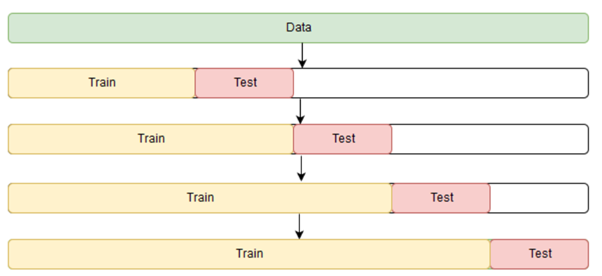
\includegraphics[width=0.62\linewidth]{1_qvdnPF8ETV9mFdMT0Y_BBA.png}
\caption{Esquema de validación con ventana expansiva. Cada partición de entrenamiento (azul)
es un superconjunto de la anterior y el bloque de validación (naranja) siempre está en el
futuro respecto a los datos con los que se ajusta el modelo.}
\label{fig:splits}
\end{figure}

\paragraph{Ausencia de fuga de información.} Se aplican tres reglas, verificadas con pruebas
automatizadas:
\begin{enumerate}
  \item Toda covariable oceanográfica es un desplazamiento de al menos $\horizonte$ días, ya sea
  del valor o de una media móvil que termina en $t$ y luego se desplaza.
  \item Toda estadística agregada ---medias y desviaciones de estandarización, estadísticas de
  imputación, los cuantiles del conformal--- se calcula \emph{únicamente} sobre el conjunto de
  entrenamiento (o de calibración) y se aplica al de prueba.
  \item En el ensamble, la predicción de un modelo que alimenta a otro se construye fuera de
  muestra con la ventana expansiva; usar la predicción en muestra le daría al segundo modelo
  una señal que en prueba no existe con esa calidad.
\end{enumerate}

\section{Métricas}
\label{sec:met_metricas}

Sean $y_1,\ldots,y_n$ las observaciones del conjunto de prueba y $\hat{y}_1,\ldots,\hat{y}_n$
las predicciones puntuales.

\paragraph{Error diario.}
\begin{align}
  \mathrm{MAE} &= \frac{1}{n}\sum_{i=1}^{n} |y_i - \hat{y}_i|, &
  \mathrm{RMSE} &= \sqrt{\frac{1}{n}\sum_{i=1}^{n} (y_i - \hat{y}_i)^2 }.
\end{align}
El MAE está en kilogramos y es interpretable; el RMSE penaliza más los errores grandes, que en
esta serie ocurren en los días de apertura.

\paragraph{Error porcentual simétrico.} Como la escala varía en dos órdenes de magnitud entre
\UEs{}, se agrega el sMAPE \citep{hyndman2006}, acotado en $[0, 200]$ y definido con la convención de que los
términos $0/0$ (día sin captura predicho como cero) cuentan como cero:
\begin{equation}
  \mathrm{sMAPE} = \frac{100}{n} \sum_{i=1}^{n}
  \frac{2\,|y_i - \hat{y}_i|}{|y_i| + |\hat{y}_i|}.
\end{equation}

\paragraph{Error en la suma de temporada.} Es la métrica que le importa a la cooperativa:
\begin{equation}
  e(\mathcal{T}_k) = 100 \cdot
  \frac{\sum_{t \in \mathcal{T}_k}\hat{y}(t) - \sum_{t \in \mathcal{T}_k} y(t)}
       {\sum_{t \in \mathcal{T}_k} y(t)} .
\end{equation}
Se reporta con signo, porque sobre-predecir y sub-predecir tienen consecuencias operativas
distintas.

\paragraph{Diagnóstico de forma.} En una serie donde la mayoría de los días están en veda, un
pronóstico casi plano obtiene un MAE bajo sin informar nada. Para distinguir el ajuste real del
aplanamiento se reportan dos diagnósticos: la razón de dispersión
$\mathrm{sd}(\hat{y})/\mathrm{sd}(y)$ ---cercana a $0$ delata un pronóstico plano, muy por
encima de $1$ un modelo que sobre-reacciona--- y la correlación de Pearson entre $\hat{y}$ y
$y$.

\paragraph{Métricas probabilísticas.} Para un cuantil $\tau \in (0,1)$ con predicción
$\hat{q}_\tau$, la pérdida \emph{pinball} es
\begin{equation}
  L_\tau(y, \hat{q}_\tau) =
  \begin{cases}
    \tau\,(y - \hat{q}_\tau) & \text{si } y \geq \hat{q}_\tau,\\
    (1-\tau)\,(\hat{q}_\tau - y) & \text{en otro caso.}
  \end{cases}
\end{equation}
El CRPS \citep{gneiting2007} se aproxima a partir de una rejilla de $m$ cuantiles mediante su
descomposición en pérdidas pinball,
\begin{equation}
  \mathrm{CRPS} \approx \frac{2}{m}\sum_{j=1}^{m} L_{\tau_j}(y, \hat{q}_{\tau_j}),
\end{equation}
y está en kilogramos, por lo que solo es comparable entre series de escala similar. Para un
intervalo $[\ell_i, u_i]$ de nivel nominal $1-\alpha$ se reportan la \textbf{cobertura
empírica} y el \textbf{ancho medio}:
\begin{align}
  \widehat{C} &= \frac{1}{n}\sum_{i=1}^{n} \mathbf{1}\{\ell_i \leq y_i \leq u_i\}, &
  \overline{W} &= \frac{1}{n}\sum_{i=1}^{n} (u_i - \ell_i).
\end{align}
Las dos se leen juntas: la cobertura sola se maximiza con un intervalo infinitamente ancho.

\section{Modelos}
\label{sec:met_modelos}

\subsection{Modelos de referencia}
ARIMA \citep{box2015} y Prophet \citep{taylor2017} sirven de piso: son autorregresivos y no usan covariables
oceanográficas, de modo que superarlos es la condición mínima para afirmar que las variables
del océano aportan señal. Los órdenes $(p,d,q)$ de ARIMA se eligen por AIC sobre el conjunto de
entrenamiento en una rejilla acotada.

\subsection{Ensambles de árboles}
XGBoost \citep{chen2016} y LightGBM \citep{ke2017} son las familias de referencia para datos
tabulares: manejan no linealidades, interacciones y valores faltantes de forma nativa, lo que
importa porque las covariables oceanográficas tienen huecos.

\subsection{Modelos recurrentes}
La LSTM \citep{hochreiter1997,greff2017,staudemeyer2019} procesa la serie como secuencia. Se usa una ventana
de 10 pasos y dos capas apiladas con \emph{dropout}. Al ser un modelo de la primera iteración
del trabajo, se conserva su arquitectura para poder comparar contra ella.

\subsection{Modelo global con la variable objetivo normalizada}
\label{sec:met_global}
El modelo global agrupa todas las series con la identidad de la serie codificada como variable
categórica. El problema del agrupamiento directo es que la función de pérdida queda dominada
por las series de mayor tonelaje. Para evitarlo se transforma la variable objetivo con
\begin{equation}
  \tilde{y} = \log(1+y),
\end{equation}
una transformación global, invertible y \emph{sin parámetros estimados} ---por lo que no puede
filtrar información del conjunto de prueba---, y se invierte con $\exp(\tilde{y})-1$ antes de
calcular cualquier métrica en kilogramos. Se comparó también la estandarización por serie
($z$-score con media y desviación calculadas solo en entrenamiento), que resulta inferior.

\subsection{Transformer de fusión temporal}
El TFT \citep{lim2021,vaswani2023} es un modelo de atención multi-horizonte con selección de
variables, diseñado para series con covariables estáticas, conocidas y observadas. Se incluye
como \emph{prueba de techo}: no como candidato a producto, sino para responder si la capacidad
adicional compra algo con este volumen de datos.

\section{Pronóstico probabilístico: regresión cuantílica conformalizada}
\label{sec:met_cqr}

El producto no es un número sino un intervalo con cobertura verificable. El procedimiento
combina regresión cuantílica con predicción conformal por partición (\emph{Mondrian}), y opera
en la escala logarítmica de la Sección~\ref{sec:met_global}:

\begin{enumerate}
  \item \textbf{Partición.} El conjunto anterior al corte se divide cronológicamente en
  \emph{entrenamiento} $\mathcal{D}_{\text{tr}}$ y \emph{calibración}
  $\mathcal{D}_{\text{cal}}$, disjuntos. La calibración se restringe a días en temporada,
  porque es el régimen en el que el intervalo se va a usar.

  \item \textbf{Cuantiles base.} Sobre $\mathcal{D}_{\text{tr}}$ se ajusta un modelo global
  cuantílico (\emph{gradient boosting} con pérdida pinball) para una rejilla de cuantiles
  $\tau_1 < \cdots < \tau_m$, obteniendo $\hat{q}_{\tau}(\cdot)$. Si los cuantiles estimados se
  cruzan, se reordenan de forma monótona por fila \citep{chernozhukov2010}.

  \item \textbf{Puntuaciones de no conformidad.} Para el intervalo de nivel $1-\alpha$ con
  cuantiles inferior $\tau_{\text{lo}} = \alpha/2$ y superior $\tau_{\text{hi}} = 1-\alpha/2$,
  se calcula en cada punto de calibración
  \begin{equation}
    E_i = \max\big\{\, \hat{q}_{\tau_{\text{lo}}}(\mathbf{x}_i) - \tilde{y}_i,\;
                       \tilde{y}_i - \hat{q}_{\tau_{\text{hi}}}(\mathbf{x}_i) \,\big\},
    \label{eq:cqr_score}
  \end{equation}
  que es positiva cuando la observación cae fuera del intervalo y negativa cuando cae dentro
  con holgura \citep{romano2019}.

  \item \textbf{Corrección.} Sea $Q_{1-\alpha}(E)$ el cuantil empírico $(1-\alpha)(1+1/|
  \mathcal{D}_{\text{cal}}|)$ de las puntuaciones. El intervalo conformalizado es
  \begin{equation}
    \Big[\, \hat{q}_{\tau_{\text{lo}}}(\mathbf{x}) - Q_{1-\alpha}(E),\;\;
            \hat{q}_{\tau_{\text{hi}}}(\mathbf{x}) + Q_{1-\alpha}(E) \,\Big],
  \end{equation}
  que bajo intercambiabilidad tiene cobertura marginal de al menos $1-\alpha$ en muestra
  finita. Se probó también una variante \emph{normalizada}, en la que la corrección se ensancha
  proporcionalmente a la dispersión local en lugar de ser constante.

  \item \textbf{Mondrian por serie.} Los pasos 3 y 4 se ejecutan \emph{por serie}: cada
  especie $\times$ \ue{} tiene su propio $Q_{1-\alpha}(E)$. Esto es indispensable porque las
  escalas difieren en órdenes de magnitud, y además permite auditar la cobertura serie por
  serie ---la cobertura marginal promedia y puede ocultar una serie mal calibrada, como se verá
  en la Sección~\ref{sec:res_cqr}.

  \item \textbf{Regreso a kilogramos.} Los extremos se invierten con $\exp(\cdot)-1$ y se
  truncan en cero. La inversión es monótona, de modo que preserva la cobertura.
\end{enumerate}

\section{Selección de hiperparámetros}
\label{sec:met_hiperparametros}

Para los modelos estadísticos se usa búsqueda exhaustiva en una rejilla acotada con criterio
AIC. Para los modelos de aprendizaje de máquina y profundo se usa optimización bayesiana con
Optuna \citep{akiba2019}, con un número limitado de ensayos para que el experimento sea
reproducible en un tiempo razonable, y evaluando siempre sobre la ventana expansiva de
validación descrita en la Sección~\ref{sec:met_particion}, nunca sobre el conjunto de prueba.
Toda componente estocástica ---inicialización de pesos, submuestreo, semillas del optimizador---
usa una semilla fija que se registra junto con las métricas del experimento.

\section{Reproducibilidad}
\label{sec:met_reproducibilidad}

El trabajo se implementó como un paquete de Python ---sobre \texttt{numpy} \citep{harris2020}, \texttt{pandas} \citep{mckinney2010}, \texttt{scikit-learn} \citep{pedregosa2011} y \texttt{PyTorch} \citep{paszke2019}--- con pruebas automatizadas
(\texttt{137} pruebas unitarias que cubren el proceso de datos, las métricas, la construcción
de variables sin fuga de información y la envoltura conformal). Cada experimento:

\begin{itemize}
  \item se ejecuta con \emph{un} comando y acepta el corte de prueba como parámetro;
  \item escribe sus métricas en un archivo JSON versionado por corte, sus figuras en PNG y un
  resumen en Markdown, de modo que ninguna cifra de este documento se transcribe a mano;
  \item fija y registra la semilla aleatoria.
\end{itemize}

Las decisiones de diseño no triviales ---el tratamiento de la variable objetivo faltante y la
justificación de la prueba de techo con el TFT--- están registradas como ADR (\emph{Architecture
Decision Records}) en el repositorio, escritas \emph{antes} de correr los experimentos
correspondientes.

\chapter{Datos}
\label{cap:datos}

Este capítulo describe de dónde vienen los datos, cómo se consolidan y qué contiene el conjunto
resultante. La descripción variable por variable está en el Apéndice~\ref{ap:variables}.

\section{Fuentes}
\label{sec:datos_fuentes}

\paragraph{Arribos pesqueros.} La variable objetivo proviene de dos fuentes complementarias.
La primera es el registro histórico de COBI (2016-2021), obtenido por convenio, con
granularidad de aviso de arribo. La segunda son los \emph{avisos de cosecha} de CONAPESCA
(``AVISOS MAYORES/MENORES DE COSECHA'', 2022-2026), publicados como datos abiertos
\citep{conapesca_datos}. La segunda fuente fue la
que permitió duplicar el número de temporadas disponibles.

\paragraph{Oceanografía.} La temperatura superficial del mar (SST) proviene del producto
reprocesado L4 de Copernicus Marine Service (OSTIA,
\texttt{METOFFICE-GLO-SST-L4-REP-OBS-SST}), con cobertura diaria global desde 1981. OSTIA es un
análisis que combina observaciones satelitales e in situ en una malla libre de nubes
\citep{donlon2012}, en la configuración operativa descrita por \citet{good2020}. Las
variables de color del océano ---clorofila (CHL), coeficiente de atenuación difusa (KD490),
materia particulada en suspensión (SPM), profundidad de disco de Secchi (ZSD), retrodispersión
de partículas (BBP) y materia orgánica coloreada disuelta (CDM)--- provienen del acervo
GlobColour \citep{globcolour2020} redistribuido por Copernicus, a 4~km de resolución.

\paragraph{Nota sobre el acceso a GlobColour.} La primera iteración de este trabajo descargaba
GlobColour por FTP. Esa vía entrega archivos \emph{globales sin recorte} (18~MB por variable y
por día a 4~km, del orden de cientos de gigabytes para el periodo y las variables de interés),
lo que la hace inviable. Se optó por la misma información redistribuida por Copernicus, que
permite recortar del lado del servidor. Las variables atmosféricas del acervo original (POC,
PIC, PAR, aerosoles, nubosidad) no están disponibles por esa vía y se omiten.

\section{Consolidación}
\label{sec:datos_etl}

Se reescribió el proceso ETL de forma modular y reproducible. Los arribos pesqueros se ingieren con granularidad de una fila por (fecha, especie, unidad económica) uniendo dos fuentes complementarias: el export histórico de COBI (2016-2021) y los avisos de cosecha (``AVISOS MAYORES/MENORES DE COSECHA'') de CONAPESCA (2022-2026). La unión se resuelve por prioridad temporal ---COBI hasta el 31-diciembre-2021 y CONAPESCA a partir de 2022, cada archivo acotado a su propio año--- de modo que no hay doble conteo en la costura de 2021. El lector de CSV autodetecta el encabezado (el preámbulo de los avisos varía entre 2 y 4 líneas) y la limpieza acepta rangos de fecha explícitos. El conjunto consolidado cubre así 2017-2026, casi duplicando las temporadas disponibles de langosta en San Quintín (de $\sim$5 a $\sim$9). Como fuente de temperatura superficial del mar (SST) se adoptó el producto reprocesado L4 de Copernicus Marine Service (OSTIA, \texttt{METOFFICE-GLO-SST-L4-REP-OBS-SST}), con cobertura diaria global desde 1981; se descargó la serie 1982-2025 y se promedió sobre el bounding box costero de cada unidad económica. Esta fuente reemplaza al cliente \texttt{motuclient} —descontinuado en 2024— por el nuevo SDK \texttt{copernicusmarine}, y provee la profundidad histórica necesaria para construir una climatología de referencia de 30 años.


\paragraph{Consistencia del empalme.} Como las dos fuentes de arribos se unen en la frontera de
2021, se verificó que la costura no introdujera un salto de escala. No hay fechas duplicadas;
COBI termina el 31-diciembre-2021 ---truncando la temporada 2021-2022 a unas 31~t--- y la unión
recupera enero y febrero de 2022, completando esa temporada a 39.5~t. La transición es continua:
diciembre de 2021 según COBI (6.3~t) es comparable con enero de 2022 según CONAPESCA (6.5~t).
La limitación honesta es que \emph{no existe un periodo de solape} entre ambas fuentes que
permita validar la escala de forma exhaustiva; el traspaso diciembre$\to$enero es la evidencia
disponible y es consistente.

\paragraph{Esquema.} El conjunto consolidado tiene una fila por
$(\text{fecha}, \text{especie}, \text{\ue{}})$ sobre el rango de fechas completo ---no solo los
días con registro---, con la variable objetivo, las covariables oceanográficas, el indicador de
temporada, la temporada a la que pertenece el día, banderas de imputación y metadatos de
trazabilidad del proceso. Se almacena en formato Parquet particionado por especie y año.

\section{Tratamiento de la variable objetivo faltante}
\label{sec:datos_faltantes}

Como el conjunto cubre todos los días y no solo los días con aviso, hay que decidir qué valor
toma la captura en los huecos. La semántica importa: un $0$ afirma ``no se pescó'' y un valor
faltante afirma ``no sabemos''. La decisión adoptada distingue tres casos:

\begin{enumerate}
  \item \textbf{Fuera de temporada} sin registro $\Rightarrow y = 0$. No es una imputación sino
  la consecuencia lógica de la veda.
  \item \textbf{Dentro de temporada} sin registro $\Rightarrow y$ faltante. Puede ser un día sin
  pesca (clima, festivo) o un hueco de captura de datos, y no hay forma de distinguirlos, así
  que no se inventa un valor.
  \item Cualquier imputación explícita queda marcada con una bandera, de modo que sea
  rastreable. No se hace por omisión.
\end{enumerate}

Cada modelo decide cómo tratar el faltante en su propia capa de preparación ---en los
experimentos de este trabajo se rellena con cero dentro de temporada, bajo el supuesto de que un
día en temporada sin registro es un día sin captura--- pero el conjunto de datos preserva la
distinción. La decisión está documentada como ADR en el repositorio.

\section{Zona de cada \ue{}}
\label{sec:datos_zona}

La oceanografía se agrega espacialmente sobre la zona costera de cada \ue{}. Lo correcto sería
recortar con el polígono TURF exacto de cada cooperativa, pero esos polígonos no son de acceso
público y no fue posible obtenerlos. Se usa en su lugar un rectángulo costero (\emph{bounding
box}) por clúster de cooperativas. A la resolución de los productos satelitales empleados
---0.25\textdegree{} para la SST y 4~km para el color del océano--- el rectángulo es una
aproximación razonable, y es además lo que hacía la primera iteración del trabajo; el polígono
exacto queda como mejora deseable y no bloqueante. La Figura~\ref{fig:mapa_ues} muestra las
zonas sobre el campo medio de SST, y la Figura~\ref{fig:zona_pesca} el detalle de la zona de
San Quintín.

\begin{figure}[htbp]
\centering
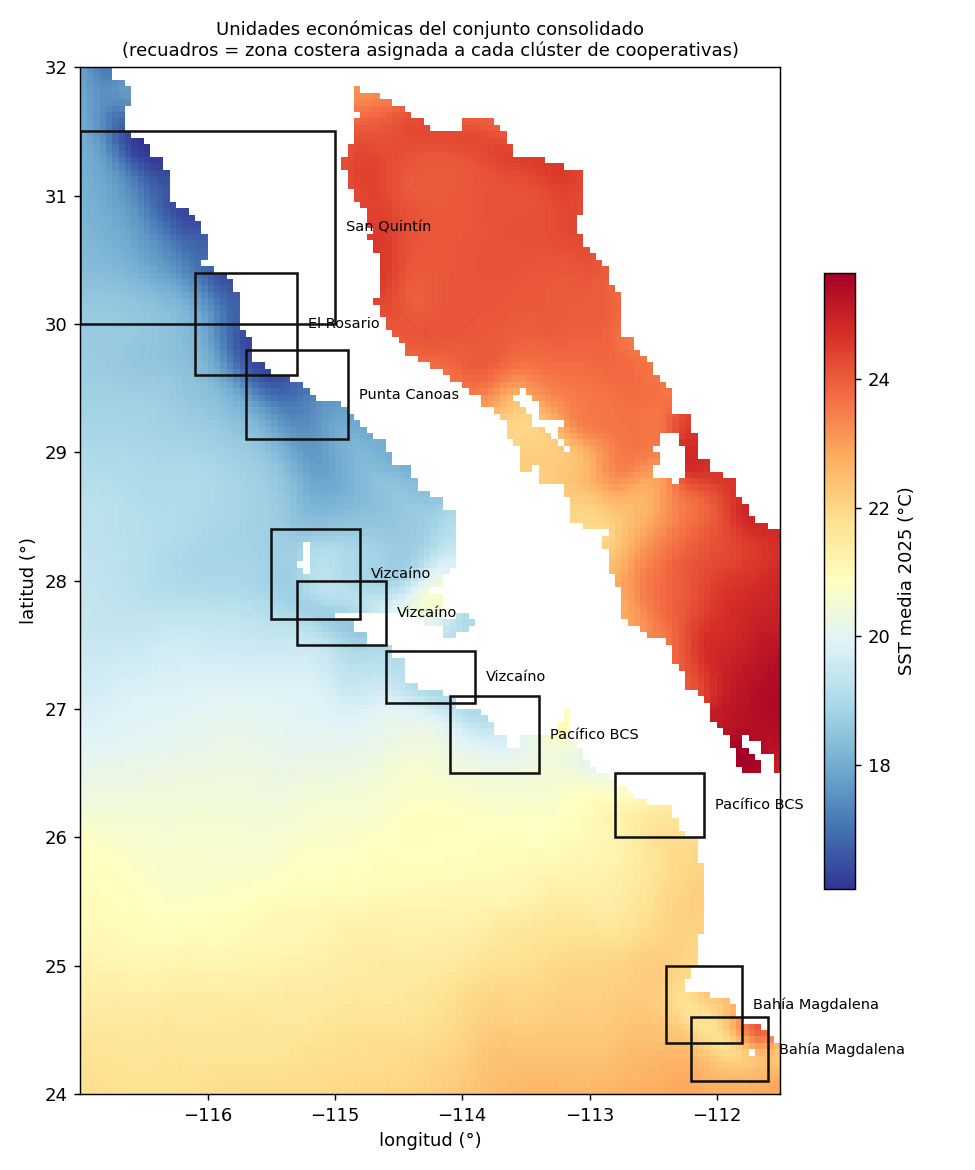
\includegraphics[width=0.78\linewidth]{mapa_ues.png}
\caption{Zonas costeras asignadas a los clústeres de \UEs{} del conjunto consolidado, sobre la
SST media de 2025. La península de Baja California aparece en blanco (sin dato de SST sobre
tierra) y el agua cálida al oriente es el Golfo de California. El gradiente térmico a lo largo
del rango es explícito: de $\sim$17\textdegree{}C en San Quintín ($\sim$30.4\textdegree{}N) a
$\sim$22\textdegree{}C en Bahía Magdalena ($\sim$24.5\textdegree{}N).}
\label{fig:mapa_ues}
\end{figure}

\section{Índice de olas de calor marinas}
\label{sec:datos_mhw}

Se implementó el índice de MHW siguiendo la metodología de Hobday et al. \cite{hobday2016}: para cada día del año se calcula una climatología y su percentil 90 sobre el periodo base 1982-2011; un evento MHW es un tramo de al menos 5 días consecutivos con SST por encima de ese umbral (fusionando eventos separados por huecos de $\leq 2$ días), y se clasifica en categorías I-IV según cuántos múltiplos de la diferencia (umbral $-$ media) alcanza la anomalía. El dataset consolidado incorpora tres columnas nuevas: \texttt{sst\_anomaly} (siempre), \texttt{mhw\_category} (0-4) y \texttt{mhw\_intensity} (definida durante eventos).

Como validación, el índice reproduce con nitidez los eventos conocidos del Pacífico nororiental: el llamado ``Blob'' de 2014-2016 (con 231, 293 y 102 días de MHW respectivamente en la zona de San Quintín) y el régimen cálido de 2019-2021 (Figura \ref{fig:mhw_timeline}). Esta validación es relevante porque conecta directamente con el mecanismo documentado por \cite{villasenor2024}.

\begin{figure}[htbp]
\centering
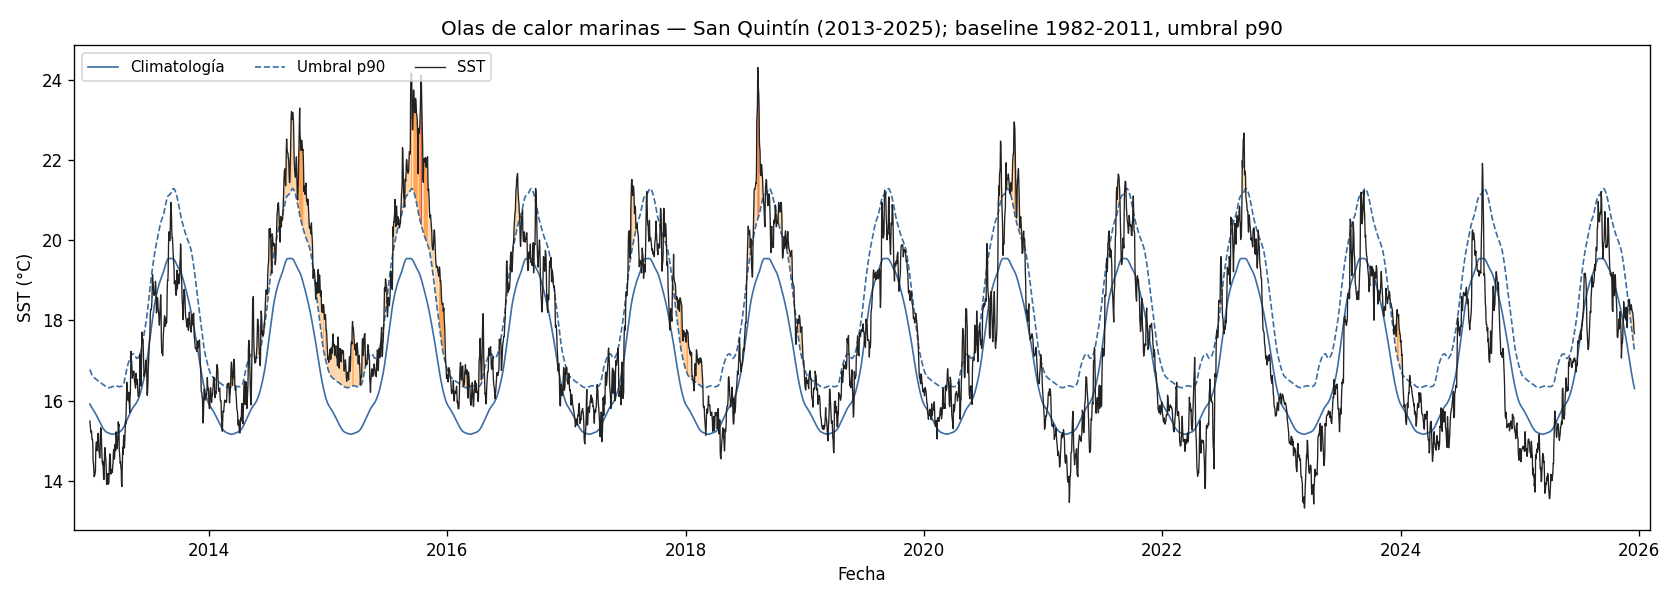
\includegraphics[width=\linewidth]{mhw_timeline.png}
\caption{Serie diaria de SST en el bbox de San Quintín (negro) contra su climatología (azul continuo) y el umbral del percentil 90 (azul discontinuo), con baseline 1982-2011 (Hobday et al. 2016). Las áreas sombreadas marcan los eventos de ola de calor marina. Destacan el ``Blob'' de 2014-2016 y el régimen cálido de 2019-2021 que precede al colapso de la captura de langosta de la temporada 2021-2022.}
\label{fig:mhw_timeline}
\end{figure}


\section{Construcción de variables}
\label{sec:datos_features}

A partir del conjunto consolidado se construye la matriz de variables explicativas de la
ecuación~\eqref{eq:problema}, con tres bloques:

\begin{itemize}
  \item \textbf{Calendario} (determinista en $t$): día del año codificado como $(\sin, \cos)$ e
  indicador de temporada.
  \item \textbf{Rezagos de la propia serie}: la captura de la misma fecha de uno y dos años
  atrás, que captura el ciclo anual.
  \item \textbf{Oceanografía desplazada}: cada covariable oceanográfica en $t-\horizonte$, más
  medias móviles de 90 y 365 días que terminan en $t-\horizonte$ ---es decir, el estado del mar
  previo a la temporada y el calor acumulado del año anterior. El desplazamiento es el mecanismo
  ecológico que se quiere modelar y, a la vez, lo que garantiza que no haya fuga de información
  (Figura~\ref{fig:desplazamiento}).
\end{itemize}

Con las seis variables de color del océano el conjunto crece a unas 35 variables, un número
grande frente a las pocas temporadas disponibles; el Capítulo~\ref{cap:resultados} muestra que
ese desbalance importa y cómo se corrige con selección de variables.

\section{El conjunto consolidado}
\label{sec:datos_resumen}

El resultado cubre \textbf{2017-2026} y contiene \textbf{44 series} (especie $\times$ \ue{}) con
al menos un día de captura registrado, que suman \textbf{10{,}465 toneladas} desembarcadas: 21
series de langosta roja (7{,}569~t), 14 de abulón azul, 6 de erizo rojo y 3 de otras especies de
abulón. La mediana de días con captura por serie es de \textbf{70}, lo que ilustra el problema
de fondo: aun con casi una década de cobertura, cada serie individual aporta pocas
observaciones. La Tabla~\ref{tab:series_resumen} desglosa cada serie.

% Generado por experiments/thesis_assets.py — no editar a mano.
\begin{longtable}{llrrrrc}
\caption{Series (especie $\times$ unidad económica) del conjunto consolidado 2017-2026. `Temporadas' cuenta las que tienen al menos un día de captura; la cobertura es la fracción de días con el valor oceanográfico disponible.}\label{tab:series_resumen}\\
\toprule
Especie & Zona & Temporadas & Días con captura & Toneladas & Cobertura SST & Cobertura CHL \\
\midrule
\endfirsthead
\toprule
Especie & Zona & Temporadas & Días con captura & Toneladas & Cobertura SST & Cobertura CHL \\
\midrule
\endhead
\bottomrule
\endfoot
Abulón negro & San Quintín (LITORAL DE BAJA CALIFO) & 5 & 51 & 2.5 & 100\% & 100\% \\
Abulón negro & El Rosario (SCPP ENSENADA SCL) & 5 & 20 & 2.3 & 100\% & 100\% \\
Abulón azul & Vizcaíno (SCPP PESCADORES NACION) & 4 & 33 & 175.1 & 100\% & 100\% \\
Abulón azul & El Rosario (SCPP ENSENADA SCL) & 9 & 68 & 59.7 & 100\% & 100\% \\
Abulón azul & Pacífico BCS (SCPP LA PURISIMA SC DE) & 4 & 28 & 24.8 & 100\% & 100\% \\
Abulón azul & Bahía Magdalena (SCPP PUERTO CHALE SCL) & 4 & 15 & 16.2 & 100\% & 100\% \\
Abulón azul & Vizcaíno (SCPP BAHIA TORTUGAS SC) & 1 & 8 & 9.3 & 100\% & 100\% \\
Abulón azul & Punta Canoas (SPR PUNTA CANOAS S DE ) & 9 & 31 & 7.8 & 100\% & 100\% \\
Abulón azul & San Quintín (LITORAL DE BAJA CALIFO) & 5 & 62 & 5.5 & 100\% & 100\% \\
Abulón azul & Pacífico BCS (SC PROGRESO DE PRODUCC) & 4 & 17 & 5.1 & 100\% & 100\% \\
Abulón azul & Bahía Magdalena (SCPP BAHIA MAGDALENA S) & 1 & 6 & 4.2 & 100\% & 100\% \\
Abulón azul & Pacífico BCS (SCPP CALIFORNIA DE SAN) & 1 & 5 & 2.6 & 100\% & 100\% \\
Abulón azul & Vizcaíno (SCPP BUZOS Y PESCADORE) & 3 & 4 & 2.6 & 100\% & 100\% \\
Abulón azul & Vizcaíno (SCPP EMANCIPACION SC D) & 4 & 12 & 2.1 & 100\% & 100\% \\
Abulón azul & Pacífico BCS (SCPP PUNTA ABREOJOS SC) & 1 & 2 & 0.3 & 100\% & 100\% \\
Abulón azul & El Rosario (SPR ASOCIACION PESQUER) & 1 & 1 & 0.0 & 100\% & 100\% \\
Abulón rojo & San Quintín (LITORAL DE BAJA CALIFO) & 5 & 42 & 2.9 & 100\% & 100\% \\
Langosta roja & El Rosario (SCPP ENSENADA SCL) & 10 & 688 & 1,181.2 & 100\% & 100\% \\
Langosta roja & Vizcaíno (SCPP PESCADORES NACION) & 10 & 307 & 904.2 & 100\% & 100\% \\
Langosta roja & Vizcaíno (SCPP BAHIA TORTUGAS SC) & 5 & 193 & 767.1 & 100\% & 100\% \\
Langosta roja & San Quintín (LITORAL DE BAJA CALIFO) & 9 & 1110 & 689.7 & 100\% & 100\% \\
Langosta roja & Vizcaíno (SCPP EMANCIPACION SC D) & 5 & 182 & 615.8 & 100\% & 100\% \\
Langosta roja & Pacífico BCS (SCPP LA PURISIMA SC DE) & 5 & 78 & 532.9 & 100\% & 100\% \\
Langosta roja & Vizcaíno (SCPP LEYES DE REFORMA ) & 6 & 148 & 493.8 & 100\% & 100\% \\
Langosta roja & Pacífico BCS (SC PROGRESO DE PRODUCC) & 6 & 133 & 366.5 & 100\% & 100\% \\
Langosta roja & Vizcaíno (SCPP BUZOS Y PESCADORE) & 5 & 143 & 362.1 & 100\% & 100\% \\
Langosta roja & El Rosario (PESCADORES EL CHUTE SP) & 10 & 307 & 282.4 & 100\% & 100\% \\
Langosta roja & El Rosario (ASOCIACION PESQUERA MO) & 10 & 269 & 267.7 & 100\% & 100\% \\
Langosta roja & Pacífico BCS (SCPP PUNTA ABREOJOS SC) & 5 & 109 & 260.2 & 100\% & 100\% \\
Langosta roja & El Rosario (SPR ASOCIACION PESQUER) & 10 & 392 & 232.4 & 100\% & 100\% \\
Langosta roja & El Rosario (ISLA SAN GERONIMO SPR ) & 10 & 316 & 162.3 & 100\% & 100\% \\
Langosta roja & Pacífico BCS (SCPP CALIFORNIA DE SAN) & 5 & 67 & 152.0 & 100\% & 100\% \\
Langosta roja & Punta Canoas (SPR PUNTA CANOAS S DE ) & 10 & 208 & 82.6 & 100\% & 100\% \\
Langosta roja & San Quintín (EL PABELLON DE SAN QUI) & 8 & 193 & 80.0 & 100\% & 100\% \\
Langosta roja & San Quintín (ROCAS DE SAN MARTIN SP) & 10 & 217 & 58.3 & 100\% & 100\% \\
Langosta roja & Bahía Magdalena (SCPP PUERTO CHALE SCL) & 5 & 44 & 34.2 & 100\% & 100\% \\
Langosta roja & Bahía Magdalena (SCPP BAHIA MAGDALENA S) & 6 & 72 & 25.3 & 100\% & 100\% \\
Langosta roja & Bahía Magdalena (SCPP PUERTO SAN CARLOS) & 5 & 89 & 18.8 & 100\% & 100\% \\
Erizo rojo & El Rosario (SCPP ENSENADA SCL) & 10 & 490 & 1,483.3 & 100\% & 100\% \\
Erizo rojo & El Rosario (SPR ASOCIACION PESQUER) & 10 & 487 & 644.6 & 100\% & 100\% \\
Erizo rojo & El Rosario (ASOCIACION PESQUERA MO) & 10 & 406 & 406.5 & 100\% & 100\% \\
Erizo rojo & El Rosario (PESCADORES EL CHUTE SP) & 4 & 21 & 19.2 & 100\% & 100\% \\
Erizo rojo & El Rosario (ISLA SAN GERONIMO SPR ) & 2 & 9 & 10.4 & 100\% & 100\% \\
Erizo rojo & Punta Canoas (SPR PUNTA CANOAS S DE ) & 9 & 23 & 8.4 & 100\% & 100\% \\
\end{longtable}


\section{Origen de la información de las figuras heredadas}

La primera iteración de este trabajo construyó su proceso de datos sobre GlobColour por FTP y
sobre un intercambio directo de archivos con COBI. Ese proceso se muestra en la
Figura~\ref{fig:etl_globcolour} y se conserva porque documenta el punto de partida; el proceso
vigente es el descrito en la Sección~\ref{sec:datos_etl}.

\begin{figure}[htbp]
    \centering
    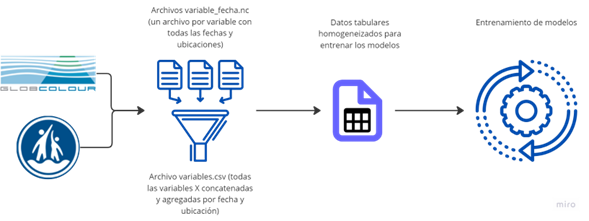
\includegraphics[width=0.95\linewidth]{Imagen1.png}
    \caption{Proceso de datos de la primera iteración del trabajo: ingesta de GlobColour por FTP
    y de los archivos de COBI, transformación de \texttt{.nc} a tablas y consolidación. El
    proceso vigente, descrito en la Sección~\ref{sec:datos_etl}, sustituye la ingesta por FTP
    por el SDK de Copernicus con recorte del lado del servidor.}
    \label{fig:etl_globcolour}
\end{figure}


\chapter{Resultados}
\label{cap:resultados}

Los resultados se presentan en el orden en que se produjeron, porque ese orden \emph{es} el
argumento: cada sección responde a una limitación descubierta en la anterior. Se parte de la
comparación de modelos puntuales sobre una sola serie, que deja abierta la pregunta del año
atípico; se identifica el mecanismo ambiental que lo explica; se intenta ---sin éxito---
resolver la escasez de datos con más variables, con selección de variables y con el agrupamiento directo;
se reformula el pronóstico en términos probabilísticos; se pone a prueba la hipótesis de datos
aumentando las series y las temporadas; y finalmente se contrasta contra una arquitectura de
vanguardia.

\section{Primera iteración: comparación de modelos puntuales}
\label{sec:res_primera}

Después de la optimización de hiperparámetros y parámetros de cada modelo, y de la toma de decisión de arquitectura en el caso de LSTM, se llegó a los modelos representativos de la Tabla~\ref{tab:modelos_seleccionados}:
\begin{table}[htbp]
\centering
\small
\begin{tabular}{lp{9.5cm}}
\toprule
Modelo & Arquitectura / Parámetros\\
\midrule
LSTM & (*) \\
Prophet & changepoint prior scale: 0.016, seasonality prior scale: 750.108 \\
LGBM & colsample bytree: 0.64, learning rate: 0.10, max depth: 6, n estimators: 63, num leaves: 67 \\
XGBoost & colsample bytree: 0.37, learning rate: 0.02,  max depth: 10, n estimators: 190 \\
ARIMA & d: 0, p: 29, q: 24, trend: c \\
\bottomrule
\end{tabular}
\caption{Modelos seleccionados y su composición}
\label{tab:modelos_seleccionados}
\end{table}


(*) La arquitectura y los hiperparámetros del modelo LSTM elegido son:

\subsubsection*{Arquitectura de la LSTM}

- Capa de entrada con dimensiones de entrada (batch size, time steps, features) igual a (None, 10, 17).

- Capa LSTM con 2700 unidades, activación 'relu', función de activación recurrente 'sigmoid', y una tasa de dropout del 30\%. Esta capa regresa secuencias y no estados.

- Capa de dropout con una tasa de dropout del 30\%, aplicada a la salida de la capa LSTM.

- Capa LSTM con 800 unidades, activación 'relu', función de activación recurrente 'sigmoid', y una tasa de dropout del 30\%. Esta capa no retorna secuencias, solo el estado final.

- Capa de dropout con una tasa de dropout del 30\%, aplicada a la salida de la segunda capa LSTM.

- Capa densa con 1 unidad y activación 'relu'.

\subsubsection*{Hiperparámetros de la LSTM}

- Unidades en la primera capa LSTM: 2700.

- Unidades en la segunda capa LSTM: 800.

- Tasa de dropout: 30\%.

- Función de activación en las capas LSTM: 'relu'.

- Función de activación recurrente en las capas LSTM: 'sigmoid'.

- Se utiliza la inicialización de pesos GlorotUniform para las capas LSTM y Dense.

- Se utiliza la inicialización de pesos Orthogonal para los pesos recurrentes de las capas LSTM.

- Las capas LSTM no son stateful y no se desenrollan en el tiempo.

- Se utiliza la implementación 2 para las capas LSTM.

- La capa densa tiene 1 unidad de salida.\\

Los resultados de las métricas de cada modelo, tal como los reportó el borrador, se resumen en la Tabla~\ref{tab:metricas_borrador}; las gráficas de valores predichos contra valores reales de cada modelo están en el Apéndice~\ref{ap:figuras} (Figuras \ref{fig:pred_arima} a \ref{fig:pred_ensemble_ambas}).

\begin{table}[htbp]
\centering
\small
\begin{tabular}{lccccc}
\toprule
Modelo & Err.\ temp.\ 2020-21 & Err.\ temp.\ 2021-22 & Err.\ ambas & RMSE & MAE \\
\midrule
XGBoost + LSTM & 8.7\% & 92\% & 12.9\% & 527.3 & 369.0 \\
XGBoost & 12\% & 16.3\% & 14.5\% & 450.7 & 312.6 \\
LGBM & 36\% & 36\% & 36.4\% & 494.9 & 380.2 \\
\midrule
LSTM & --- & --- & 61\% & 183.1 & 104.9 \\
Prophet & 164\% & 1737\% & 761\% & 135.0 & 105.8 \\
ARIMA & 338\% & 142\% & 142\% & 467.5 & 344.1 \\
\bottomrule
\end{tabular}
\caption{Resultados de la primera iteración (borrador de 2023) por modelo: error en la suma de
temporada (2020-2021, 2021-2022 y ambas) y RMSE/MAE diarios en kg. \emph{Nota}: las cifras se
transcriben tal cual del borrador, cuyo proceso de datos dependía de fuentes hoy inaccesibles y
no es reproducible; contienen inconsistencias internas menores de transcripción (algunos errores
porcentuales no cuadran exactamente con las sumas que los acompañaban), por lo que deben leerse
como el registro histórico del punto de partida y no como cifras verificadas. La re-corrida
verificable de estos mismos modelos sobre el conjunto unido 2017-2026 está en la
Tabla~\ref{tab:extension_comparativa}.}
\label{tab:metricas_borrador}
\end{table}


Se optó por ensamblar XGBoost, el mejor modelo para predecir la tendencia, junto con LSTM: primero se hace la predicción con XGBoost y ese vector de y se introduce en LSTM como un regresor más. Los resultados del ensamble son los mejores, con un error de captura del 8.7\% para la primera temporada y un error global del 12.9\%. A pesar de esto, los resultados para la segunda temporada no son nada favorables. 

Además, los RMSE y MAE son elevados, lo cual implica que las predicciones diarias son poco precisas, a pesar de que la suma de toda la temporada se predice con poco error. Esto puede significar un reto para confiar en el modelo, pero es consecuencia de la falta de granularidad en los datos de entrenamiento.

En general, todos los modelos sobreestimaron la pesca de la segunda temporada debido a que podría tratarse de un caso atípico. Si comparamos esta temporada con el resto, el total de pesca es menos de la mitad. Por esta razón se decidió optar por predecir la temporada 2020-2021 también, pues es similar a las demás.

No obstante, debemos poner atención a la causa de la reducción de la pesca en la temporada 2021-2022. Inicialmente se planteó la hipótesis de un efecto económico externo (el último año de la pandemia de Covid-19); sin embargo, el índice de olas de calor marinas de la Sección~\ref{sec:datos_mhw} atribuye la caída a un mecanismo ambiental: las olas de calor marinas que afectaron a Baja California entre 2019 y 2021 \citep{villasenor2024}. Esto explica por qué los modelos que solo usan el historial de capturas —o las variables oceanográficas sin un índice de anomalía térmica de largo plazo— sobreestiman sistemáticamente esa temporada.

El paso siguiente que este planteamiento dejaba señalado ---conseguir datos de otras regiones y de otras especies, replicar el procedimiento y verificar si los modelos elegidos sostienen sus resultados--- es exactamente el que emprenden las secciones que siguen.


\subsection{El bache de la temporada 2021-2022 se explica por olas de calor}
Las sumas de captura de langosta en San Quintín, reconstruidas a partir de los arribos, muestran una caída pronunciada tras el régimen cálido 2019-2021: aproximadamente 173 t en 2019-2020, 106 t en 2020-2021 y 39.5 t en 2021-2022 (una reducción cercana al 77\% respecto al máximo). Es más, la unión con CONAPESCA revela que la captura \emph{no se recuperó} en las temporadas siguientes, sino que se estabilizó en niveles bajos: 24.4 t en 2022-2023, 18.5 t en 2023-2024 y 17.0 t en 2024-2025 (una décima parte del máximo). Esta magnitud iguala o supera el rango de 15-58\% de reducción de capturas atribuido a las MHW en Baja California \cite{villasenor2024}, coherente con que los impactos son mayores cerca de quiebres biogeográficos como San Quintín; y resuelve la pregunta abierta de la sección de Resultados: la caída no obedece principalmente a un efecto económico, sino a un forzamiento ambiental que los modelos originales no podían anticipar por carecer de una variable de anomalía térmica de largo plazo.

Un detalle de la reconstrucción merece mención, porque valida la unión de fuentes: el registro de COBI termina el 31-diciembre-2021, a mitad de la temporada 2021-2022, de modo que por sí solo la truncaba (solo $\sim$31 t hasta diciembre). La unión con CONAPESCA recupera el tramo enero-febrero de 2022 y completa la temporada en 39.5 t. El empalme es limpio: no hay fechas duplicadas entre fuentes, y la transición es continua ---diciembre de 2021 (COBI, 6.3 t) y enero de 2022 (CONAPESCA, 6.5 t) reportan a escalas compatibles---, lo que da confianza en que comparar temporadas anteriores (COBI) con posteriores (CONAPESCA) no introduce un artefacto de fuente.

\subsection{Re-entrenamiento del baseline y modelo con covariables}
Sobre los datos reales reconstruidos (langosta $\times$ San Quintín, corte de prueba 01-julio-2020) se re-entrenaron los modelos baseline y un modelo con las nuevas covariables oceanográficas (SST y MHW desplazadas 90 días, respetando la convención del proyecto y evitando fuga de datos). La Tabla \ref{tab:extension_floor} resume el desempeño.

\begin{table}[htbp]
\centering
\small
\begin{tabular}{lccccc}
\toprule
Modelo & MAE & RMSE & sMAPE (\%) & Err.\ 2020-21 & Err.\ 2021-22 \\
\midrule
ARIMA(3,0,3) & 345 & 463 & 138 & $-26\%$ & $+291\%$ \\
Prophet & 372 & 576 & 129 & $+62\%$ & $+418\%$ \\
XGBoost (SST+MHW) & 327 & 558 & 126 & $+53\%$ & $+368\%$ \\
\bottomrule
\end{tabular}
\caption{Baseline re-derivado sobre datos reales y modelo con covariables SST/MHW. Todos sobreestiman fuertemente la temporada del bache (2021-2022).}
\label{tab:extension_floor}
\end{table}

Los modelos autorregresivos (ARIMA, Prophet), que solo usan el historial de $y$, sobreestiman la temporada 2021-2022 por factores de 3 a 4, pues no ``ven'' la ola de calor. El modelo XGBoost con covariables sí selecciona las variables de MHW entre sus más importantes (por ejemplo, la media móvil de anomalía de SST y de categoría MHW del año previo), pero con únicamente tres temporadas de entrenamiento no logra aún corregir la sobreestimación. Esto confirma el diagnóstico del trabajo original: el cuello de botella no es la complejidad del modelo, sino la escasez de temporadas.

\subsection{Color del océano y selección de variables con SHAP}
Para enriquecer el conjunto de regresoras se integraron seis variables ópticas y biológicas de color del océano, re-distribuidas por Copernicus Marine a partir del acervo GlobColour: clorofila (CHL), coeficiente de atenuación difusa (KD490), materia particulada en suspensión (SPM), profundidad de disco de Secchi (ZSD), retrodispersión de partículas (BBP) y materia orgánica coloreada disuelta y detritos (CDM). Al igual que la SST se desplazan 90 días y se agregan medias móviles, con lo que el conjunto crece a unas 35 variables. Sin embargo, añadirlas al modelo de una sola serie \emph{empeora} el desempeño (MAE de 327 a 424; error de la temporada 2021-2022 de $+368\%$ a $+399\%$): un caso claro de sobreajuste con 35 variables y solo tres temporadas.

Para verificar si el problema era el exceso de variables, se aplicó una selección basada en valores SHAP \cite{lundberg2017} (\emph{TreeExplainer}): se ordenaron las variables por su importancia media absoluta $|$SHAP$|$ y se conservaron las que aportaban al menos el 1\% del total, reduciendo de 35 a 16. El ordenamiento es coherente y físicamente interpretable ---dominan el calendario (\texttt{doy\_sin}, \texttt{in\_season}), seguido de la retrodispersión de partículas rezagada (\texttt{bbp\_roll90\_lag90}), el rezago anual de $y$ y variables de SST/color del océano---, lo que indica que las variables tienen sentido. No obstante, podar \emph{no} corrige el sobreajuste (Tabla \ref{tab:extension_shap}): el modelo reducido es incluso ligeramente peor.

\begin{table}[htbp]
\centering
\begin{tabular}{lccccc}
\toprule
Modelo & N.\ variables & MAE & RMSE & sMAPE (\%) & Error temp. 2021-22 \\
\midrule
Completo & 35 & 423.6 & 659.7 & 116.0 & $+398.7\%$ \\
Podado (SHAP) & 16 & 444.7 & 695.5 & 120.3 & $+446.6\%$ \\
\bottomrule
\end{tabular}
\caption{Selección de variables con SHAP sobre langosta $\times$ San Quintín (corte 01-julio-2020). Podar a las 16 variables de mayor $|$SHAP$|$ no mejora el desempeño: el cuello de botella no es \emph{cuáles} variables se usan, sino el volumen de datos.}
\label{tab:extension_shap}
\end{table}

La conclusión metodológica es importante: la selección de variables por sí sola no resuelve el sobreajuste, porque el factor limitante no es la dimensionalidad sino la cantidad de temporadas. Esto refuerza que la palanca real está en \emph{sumar datos} ---más unidades económicas y más temporadas---, motivando el modelo global de la siguiente sección.

\subsection{Modelo global multi-especie y multi-unidad económica}
Para atacar la escasez de datos por serie se entrenó un único modelo global sobre varias series (especie, unidad económica), con codificación one-hot de especie y de unidad económica y la oceanografía compartida, y se comparó contra modelos específicos entrenados por serie. Se incorporó una segunda unidad económica, Isla Cedros ($\sim$28$^\circ$N), además de San Quintín ($\sim$30.5$^\circ$N), lo que introduce variación a lo largo del gradiente biogeográfico. La Tabla \ref{tab:extension_global} muestra la comparación por serie.

\begin{table}[htbp]
\centering
\begin{tabular}{lccc}
\toprule
Serie (especie @ unidad económica) & RMSE global & RMSE específico & Gana \\
\midrule
langosta @ Isla Cedros & 893.6 & 898.7 & global \\
langosta @ San Quintín & 618.9 & 558.3 & específico \\
abulón negro @ San Quintín & 24.6 & 52.8 & global \\
abulón azul @ San Quintín & 24.1 & 6.0 & específico \\
abulón rojo @ San Quintín & 24.0 & 8.9 & específico \\
\bottomrule
\end{tabular}
\caption{Modelo global vs. modelos específicos, por serie (RMSE diario, kg). El global gana o empata en 2 de 5 series.}
\label{tab:extension_global}
\end{table}

De aquí surgen dos hallazgos. Primero, hay \emph{transferencia positiva dentro de una misma especie entre unidades económicas}: la langosta de Isla Cedros, con menos datos, mejora ligeramente al agruparse con la de San Quintín. Segundo, el agrupamiento indiscriminado de todas las especies en un solo modelo se ve \emph{confundido por la escala}: la langosta (capturas de cientos de kilogramos) domina la función de pérdida frente al abulón (unidades de kilogramos), degradando las predicciones de este último. La conclusión metodológica es que conviene agrupar por especie entre unidades económicas —o normalizar la variable objetivo por serie— en lugar de un pooling total, es decir, avanzar hacia un modelo jerárquico o de \emph{partial pooling}.

\subsection{Normalización de la variable objetivo por serie}
La hipótesis anterior se puso a prueba directamente. Antes de agrupar, se transformó la variable objetivo de cada serie con $\log(1+y)$ —una transformación global, invertible y sin parámetros estimados— de modo que las series de mayor volumen dejaran de dominar la función de pérdida; también se probó una estandarización ($z$-score) por serie con media y desviación calculadas únicamente sobre el conjunto de entrenamiento, para evitar fuga de información. La Tabla \ref{tab:extension_ynorm} compara, por serie, el modelo específico contra el pooling sobre la variable cruda y contra el pooling sobre $\log(1+y)$; todas las predicciones se invierten a kilogramos antes de medir el RMSE.

\begin{table}[htbp]
\centering
\small
\begin{tabular}{lccc}
\toprule
Serie (especie @ UE) & específico & pooling crudo & pooling $\log(1{+}y)$ \\
\midrule
abulón negro @ San Quintín & 52.0 & 35.4 & \textbf{7.0} \\
abulón azul @ San Quintín & 6.7 & 32.7 & \textbf{4.6} \\
abulón rojo @ San Quintín & 7.3 & 34.9 & \textbf{3.5} \\
langosta @ Isla Cedros & 914.1 & 889.0 & 1131.4 \\
langosta @ San Quintín & 659.7 & 742.2 & \textbf{544.4} \\
\bottomrule
\end{tabular}
\caption{Pooling con la variable objetivo normalizada por serie vs. modelos específicos (RMSE diario, kg, tras invertir la transformación). El pooling sobre $\log(1+y)$ gana o empata en 4 de 5 series; la estandarización por serie ($z$-score, no mostrada) resulta inferior (1 de 5). En negrita, la mejor de cada fila.}
\label{tab:extension_ynorm}
\end{table}

El resultado confirma la hipótesis: al normalizar el objetivo, el pooling \emph{sí} supera a los modelos específicos, ganando o empatando en 4 de 5 series con la transformación $\log(1+y)$, frente a solo 2 de 5 del pooling crudo. El efecto es más marcado en las series de escala pequeña —el abulón, cuyo RMSE cae de $\sim$33--35 (pooling crudo, dominado por la langosta) a 3.5--7.0 kg, por debajo incluso de su modelo específico— y también mejora la serie insignia de langosta en San Quintín (544 vs. 659 kg). La única serie que empeora es la langosta de Isla Cedros, la de mayor escala, donde el logaritmo comprime en exceso. La estandarización por serie queda por detrás del logaritmo, previsiblemente porque con pocas temporadas las estadísticas de escala por serie son ruidosas. La conclusión operativa es que el \emph{partial pooling con la variable objetivo en escala logarítmica} es el modelo global a consolidar y el candidato natural a envolver en un esquema de predicción probabilística (regresión cuantílica conformalizada) en la siguiente fase.

\subsection{Pronóstico probabilístico con regresión cuantílica conformalizada}
Con tres temporadas, cualquier pronóstico puntual es ruidoso; lo honesto ---y lo útil para una cooperativa que planea insumos--- es entregar un \emph{rango} calibrado en lugar de un solo número. Se envolvió el modelo global $\log(1+y)$ en una regresión cuantílica conformalizada (CQR, \citealp{romano2019}): regresores cuantílicos de gradient boosting en escala logarítmica y una corrección conformal de conjunto de calibración, con las cotas invertidas a kilogramos. La calibración se hace \emph{por serie} (variante de Mondrian) y \emph{solo con días en temporada}: los días fuera de temporada, con captura nula y cuantiles base cercanos a cero, tienen residuo de conformidad nulo y, por su abundancia, anulaban la corrección; restringir la calibración a la temporada la vuelve informativa. La partición temporal es estricta (calibración anterior al corte de prueba 01-julio-2020).

La Tabla \ref{tab:extension_cqr} muestra la cobertura empírica y el ancho de los intervalos. La cobertura marginal queda cerca del nivel nominal (86\% para el intervalo nominal del 90\%, 81\% para el del 80\%), y la variante \emph{normalizada} (ensanchamiento proporcional a la dispersión local) es ligeramente mejor que la de corrección constante. Es notable que la cobertura se mantiene durante las olas de calor marinas (0.89 en días de MHW frente a 0.85 fuera): el intervalo sigue siendo honesto precisamente en el régimen anómalo que hacía fracasar al pronóstico puntual.

\begin{table}[htbp]
\centering
\begin{tabular}{lcc}
\toprule
Intervalo nominal & Cobertura empírica & Cobertura en días de MHW \\
\midrule
80\% & 80.8\% & --- \\
90\% & 85.9\% & 89.1\% (vs.\ 85.4\% fuera de MHW) \\
\bottomrule
\end{tabular}
\caption{Cobertura empírica de la CQR (modelo global $\log(1+y)$, por serie, calibrada en temporada; corte 01-julio-2020). Cercana al nivel nominal y estable durante olas de calor marinas.}
\label{tab:extension_cqr}
\end{table}

La cobertura marginal, sin embargo, promedia series heterogéneas: el abulón sobre-cubre (cerca del 99\%) mientras que la langosta de San Quintín sub-cubre (alrededor del 53\%), porque la caída post-MHW de 2021-2022 lleva las capturas por debajo de la cota inferior calibrada con años previos ---un recordatorio de que, con una sola temporada de calibración, un cambio de régimen queda fuera de la distribución aprendida. La otra limitación honesta es que la cota superior de los días pico sigue siendo ancha: eso lo determina el modelo cuantílico base (el cuantil 0.95 en escala logarítmica, amplificado al exponenciar), no la envoltura conformal. Un intento de endurecer los cuantílicos base con optimización bayesiana de hiperparámetros (Optuna sobre la pérdida pinball) mejoró la validación pero empeoró notoriamente el test en las series de gran escala, al sobreajustar el periodo de validación: confirma que estrechar el intervalo requiere \emph{más temporadas}, no más maquinaria. Aun así, el producto ---un rango calibrado de captura por especie y unidad económica--- es directamente entregable a las cooperativas y constituye el resultado operativo de esta fase.

\subsection{La hipótesis de datos, puesta a prueba: más unidades y más temporadas}
\label{sec:extension_moredata}
Todos los experimentos anteriores convergen en el mismo diagnóstico ---el factor limitante es el volumen de datos, no la sofisticación del modelo---, pero lo enuncian sin demostrarlo causalmente. La forma directa de ponerlo a prueba es \emph{sumar datos} y medir si la calibración mejora. Se hizo en dos frentes.

Primero, se amplió la cobertura espacial en dos tandas. Un clúster de cinco cooperativas de El Rosario ($\sim$29.6--30.4$^\circ$N) llevó la langosta de 2 a 7 series (especie, unidad económica): con el corte canónico de 01-julio-2020 el RMSE del \emph{pooling} de langosta en San Quintín cae de 659 a 313 kg y el ancho del percentil 90 de los días pico se estrecha de $\sim$9\,776 a $\sim$3\,812 kg ---transferencia positiva dentro de la especie. Una segunda tanda añadió tres cooperativas de la costa norte con historia completa 2017-2026 ---Punta Canoas ($\sim$29.4$^\circ$N), El Pabellón de San Quintín y Rocas de San Martín ($\sim$30.4--30.5$^\circ$N)---, llevando la langosta a 10 series: en el corte de 2024 el CRPS marginal baja de 150 a 123 kg y el de la propia langosta de San Quintín de 124 a 95 kg. Sumar zonas vecinas y de régimen térmico parecido ---la señal más clara de transferencia positiva dentro de la especie--- afina el pronóstico; más adelante se verá que sumar zonas del extremo cálido del rango ya no lo hace.

Segundo, y de mayor impacto, se desbloquearon las temporadas 2022-2026 mediante la unión con los avisos de cosecha de CONAPESCA (Sección~\ref{sec:extension2026}), lo que permite mover el corte de prueba a 01-junio-2024 y dejar el bache post-MHW y las temporadas posteriores de captura reducida \emph{dentro} del entrenamiento y la calibración. Con ese corte la CQR queda bien calibrada y ---lo crucial--- de forma \emph{estable}: la langosta de San Quintín cubre 96.2\% (cobertura marginal 96.6\% para el intervalo nominal del 90\%), las series de langosta cubren entre 96\% y 100\%, y el intervalo sigue honesto durante las olas de calor (92.5\% en días de MHW frente a 96.1\% fuera).

\begin{table}[htbp]
\centering
\small
\begin{tabular}{p{4.6cm}cccc}
\toprule
 & \multicolumn{2}{c}{Langosta @ SQ, cob.\ 90\%} & Marginal & CRPS \\
\cmidrule(lr){2-3}
Pool de langosta & Corte 2020 & Corte 2024 & 2024 & marg.\ 2024 \\
 & (bache fuera) & (bache dentro) & cob.\ 90\% & \\
\midrule
7 series (El Rosario) & 40.6\% & \textbf{96.7\%} & 96.1\% & 149.8 \\
10 series (+costa norte) & 40.6\% & \textbf{96.2\%} & 96.6\% & 123.0 \\
14 series (+Vizcaíno) & 40.6\% & \textbf{96.2\%} & 96.1\% & 229.6 \\
18 series (+Abreojos--Purísima) & 40.5\% & \textbf{96.2\%} & 96.0\% & 239.4 \\
21 series (+Bahía Magdalena) & 99.9\% & \textbf{96.2\%} & 95.8\% & 216.8 \\
\bottomrule
\end{tabular}
\caption{Estabilidad de la calibración de la langosta de San Quintín frente al corte de prueba y a la composición del pool, al expandir de 7 a 21 series. Con el corte de 2024 (el bache post-ola-de-calor \emph{dentro} del entrenamiento) la cobertura del buque insignia es \emph{invariante} a añadir zonas: se mantiene en 96.2\% a lo largo de toda la expansión, y la cobertura marginal cerca del nominal ($\sim$96\%). Con el corte de 2020 (bache \emph{fuera} del entrenamiento) la cobertura es en cambio \emph{inestable} respecto a la composición del pool ---se mantuvo en $\sim$41\% hasta 18 series y saltó a $\sim$100\% solo al añadir Bahía Magdalena---, lo que confirma que ese corte es poco fiable (régimen fuera de distribución) y que el corte de referencia es el de 2024. El CRPS marginal sube al añadir las cooperativas de Vizcaíno y del Pacífico BCS ---las de mayor tonelaje, y el CRPS está en kg--- por un efecto de \emph{escala}, no de calidad: la cobertura por serie de las nuevas se mantiene alta (Bahía Magdalena 95--97\%).}
\label{tab:extension_moredata}
\end{table}

Una tercera tanda puso a prueba la \emph{robustez} del producto ante la composición del pool. Se añadieron cuatro grandes cooperativas FEDECOOP de la península de Vizcaíno (Bahía Tortugas, Punta Eugenia, Isla Natividad y Bahía Asunción, $\sim$27.1--27.9$^\circ$N, unos 2$^\circ$ al sur de San Quintín), llevando la langosta a 14 series. Como estas solo tienen historia de CONAPESCA (2022--2026, apenas dos temporadas de entrenamiento antes del corte de 2024), lo que se mide es estabilidad: la calibración de la langosta de San Quintín quedó \emph{intacta} (96.2\% en el corte de 2024, idéntica a la del pool de 10 series). La cobertura marginal se mantuvo cerca del nominal (96.1\% en 2024). Las nuevas series, de historia corta, se calibran razonablemente (91--93\% en el corte de 2024) y elevan el CRPS \emph{marginal} por su gran escala en kilogramos ---son las de mayor tonelaje del pool, con Bahía Tortugas en $\sim$767 t---, no por peor calidad probabilística. Es, una vez más, la firma de que la palanca es acumular temporadas, no añadir zonas de historia corta.

Una cuarta tanda extendió el pool $\sim$1$^\circ$ más al sur, al clúster de Punta Abreojos--La Purísima ($\sim$26.2--27.0$^\circ$N, cuatro cooperativas), lo que obligó a ampliar la descarga oceanográfica de Copernicus hacia el sur y el este. Con ello la langosta llegó a 18 series y el patrón de \emph{estabilidad} se repitió: la calibración de la langosta de San Quintín siguió intacta (96.2\% en el corte de 2024), la cobertura marginal cerca del nominal (96.0\%), y las nuevas cooperativas se calibraron entre 89\% y 100\%.

Una quinta tanda llevó el pool al extremo sur del rango de la langosta roja: tres cooperativas de Bahía Magdalena (Puerto San Carlos, Bahía Magdalena y Puerto Chalé, $\sim$24.1--25.0$^\circ$N), en el borde biogeográfico cálido donde la SST media supera en $\sim$4$^\circ$C a la de San Quintín; incorporarlas obligó a extender de nuevo la descarga de Copernicus hacia el sur (hasta 24$^\circ$N). Con ellas la langosta llegó a 21 series. De nuevo la calibración de San Quintín quedó intacta en el corte de 2024 (96.2\%) y las nuevas series ---pese a su historia corta--- se calibraron bien (95--97\%). Pero esta tanda marca también el \emph{límite honesto} de la transferencia entre zonas: añadir el borde térmico cálido \emph{no} afina el pronóstico de San Quintín ---su CRPS incluso empeora, de 90 a 123 kg en el corte de 2024---, a diferencia de las zonas vecinas y de régimen similar de las primeras tandas. La transferencia positiva dentro de la especie opera entre regímenes parecidos, no desde el extremo cálido del rango. El hallazgo refuerza el diagnóstico central: lo que estabiliza la calibración es acumular \emph{temporadas} (llevar el bache al entrenamiento), más que sumar \emph{zonas} indiscriminadamente. La Figura \ref{fig:extension_cqr_grid} lo muestra serie por serie para las veintiuna unidades.

\begin{figure}[htbp]
\centering
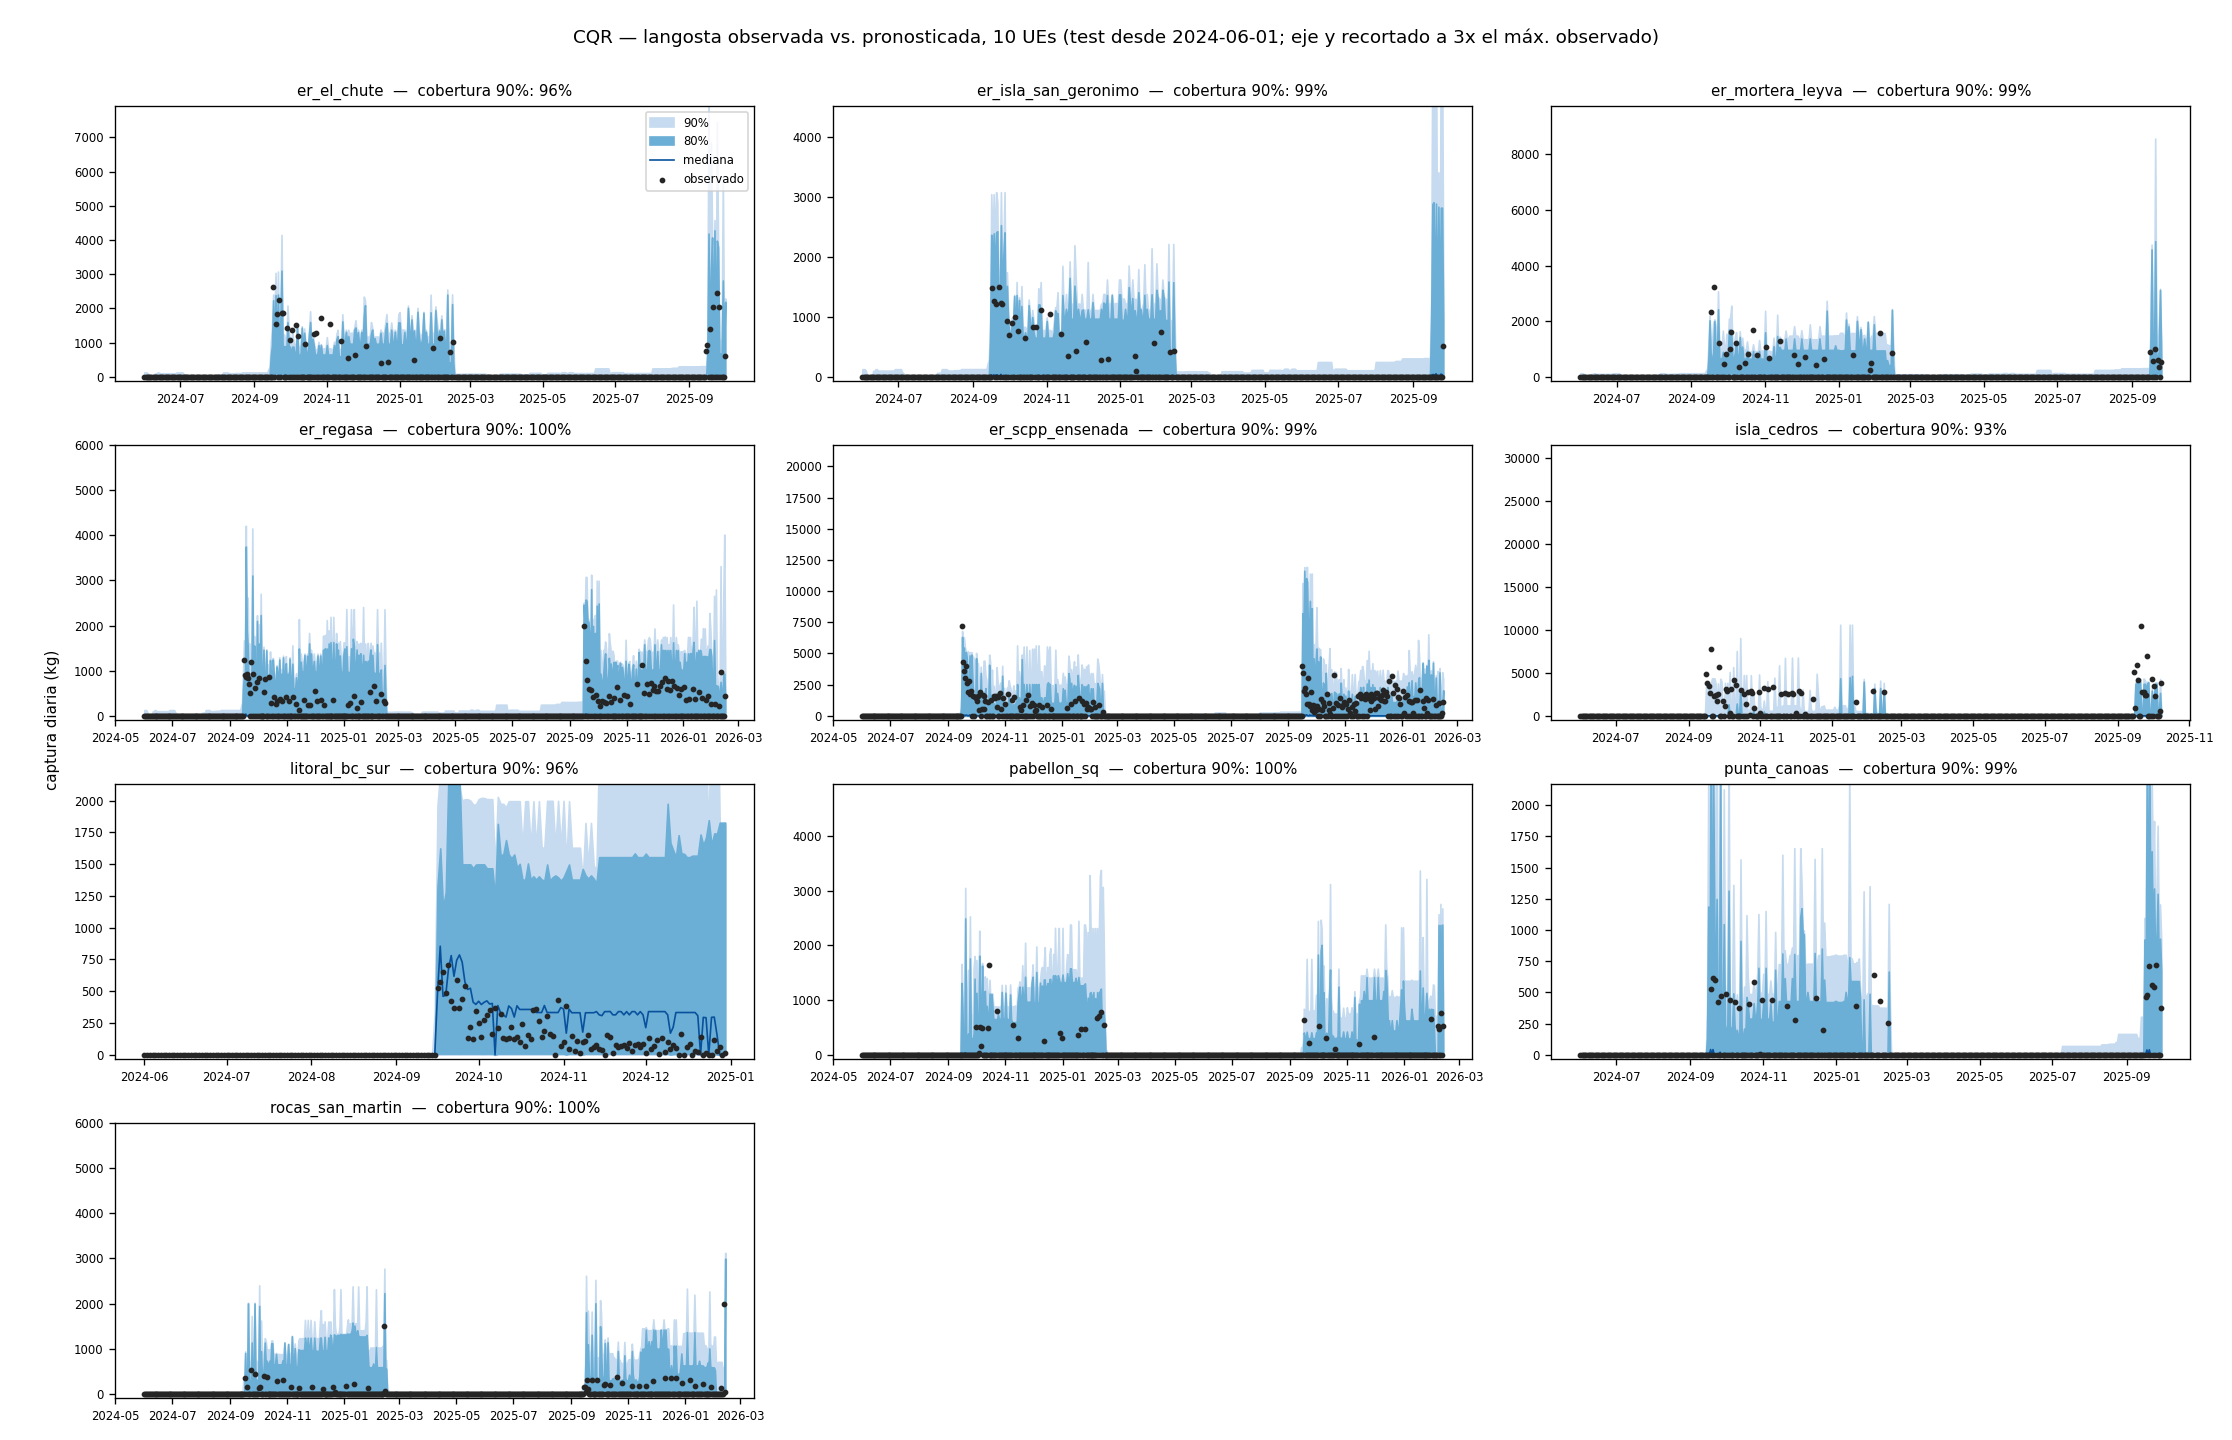
\includegraphics[width=\linewidth]{exp4_cqr_fan_grid_2024.png}
\caption{Intervalos de la CQR (bandas 80\% y 90\% + mediana) frente al observado (puntos) para las veintiuna series de langosta, en el corte 01-junio-2024. Con el bache post-ola-de-calor dentro del entrenamiento y la calibración, el observado cae dentro de las bandas de forma consistente (cobertura empírica anotada por panel, 88--100\%; las cooperativas nuevas de Vizcaíno, de solo dos temporadas de entrenamiento, en el extremo inferior), incluida la langosta de San Quintín (96.2\%). El eje $y$ de cada panel se recorta a 3$\times$ su máximo observado, pues la cota superior del 90\% se dispara en los días pico al invertir la transformación logarítmica.}
\label{fig:extension_cqr_grid}
\end{figure}

El contraste con el corte de 2020 es revelador, pero no como un simple ``antes mal, después bien''. Cuando el bache queda \emph{fuera} del entrenamiento, la cobertura por serie de la langosta de San Quintín es sencillamente \emph{poco fiable}: a lo largo de la expansión se mantuvo en $\sim$41\% desde 7 hasta 18 series y saltó a 99.9\% solo con 21 ---de la sub-cobertura severa a la sobre-cobertura severa--- sin que la serie ni su conjunto de calibración cambien, solo la composición del pool que fija el ancho del cuantil base. Es la firma de un régimen fuera de distribución: el intervalo se apoya sobre el filo de la navaja respecto a las capturas del crash. Con el bache \emph{dentro} del entrenamiento (corte 2024) la cobertura es estable (96.7\% con 7 series y 96.2\% con 10, 14, 18 y 21). Lo que compran las temporadas adicionales, entonces, no es solo un buen número de cobertura sino una calibración \emph{reproducible} ---invariante a cuántas zonas haya en el pool---, y ese es el argumento de fondo: ni la poda por SHAP ni la optimización bayesiana de los cuantílicos dieron una calibración fiable de la serie insignia; llevar el régimen anómalo al entrenamiento sí.

\subsection{Comparativa de modelos puntuales sobre datos unidos: el efecto de las temporadas de entrenamiento}
\label{sec:extension_comparativa}
Las tablas anteriores del piso (Tablas \ref{tab:extension_floor} y \ref{tab:extension_shap}) son una fotografía \emph{previa} a la unión con CONAPESCA: se calcularon con tres temporadas de entrenamiento y solo dos de prueba (2020-2022), que era todo lo que había. Con el conjunto unido 2017-2026 podemos re-entrenar los modelos puntuales de una sola serie (langosta $\times$ San Quintín) y, sobre todo, comparar de frente los dos cortes: el canónico 01-julio-2020 ($\sim$3 temporadas de entrenamiento, prueba 2020-2026 abarcando el bache y las temporadas posteriores de baja captura) contra 01-junio-2024 ($\sim$7 temporadas, con el bache \emph{dentro} del entrenamiento, prueba = temporadas recientes de baja captura). La diferencia entre columnas aísla el efecto de \emph{cuántas temporadas} ve el modelo. La Tabla \ref{tab:extension_comparativa} lo resume.

\begin{table}[htbp]
\centering
\small
\begin{tabular}{lccccccc}
\toprule
 & \multicolumn{3}{c}{Corte 2020-07-01 ($\sim$3 temp.)} & & \multicolumn{3}{c}{Corte 2024-06-01 ($\sim$7 temp.)} \\
\cmidrule(lr){2-4}\cmidrule(lr){6-8}
Modelo & MAE & RMSE & sMAPE & & MAE & RMSE & sMAPE \\
\midrule
ARIMA & 330.8 & 383.8 & 153.3 & & 177.8 & 191.5 & 147.1 \\
Prophet & 454.7 & 685.1 & 158.8 & & 190.3 & 332.0 & 64.4 \\
LGBM & 401.9 & 668.8 & 136.7 & & 153.8 & 236.2 & 124.0 \\
XGBoost (35 vars) & 459.0 & 712.3 & 153.0 & & 145.4 & 212.0 & 97.1 \\
XGBoost (SHAP, $\sim$16 vars) & 387.5 & 673.0 & 132.1 & & \textbf{103.5} & \textbf{155.6} & \textbf{64.1} \\
LSTM & 290.7 & 457.7 & 78.4 & & 499.4 & 628.7 & 131.5 \\
XGBoost+LSTM (ensamble) & \textbf{236.4} & \textbf{408.7} & \textbf{59.2} & & 561.7 & 746.6 & 115.2 \\
\bottomrule
\end{tabular}
\caption{Modelos puntuales de langosta $\times$ San Quintín re-entrenados sobre el conjunto unido 2017-2026, en los dos cortes de prueba (MAE, RMSE y sMAPE diarios, kg). En negrita, el mejor modelo de cada corte. Pasar de 3 a 7 temporadas de entrenamiento reduce el error diario a aproximadamente la mitad en los modelos tabulares ---y \emph{invierte} el orden entre ellos y los recurrentes. El ensamble XGBoost+LSTM es el del borrador original (la predicción de XGBoost entra a la LSTM como regresor extra), aquí con esa columna construida fuera de muestra en el entrenamiento.}
\label{tab:extension_comparativa}
\end{table}

\begin{figure}[htbp]
\centering
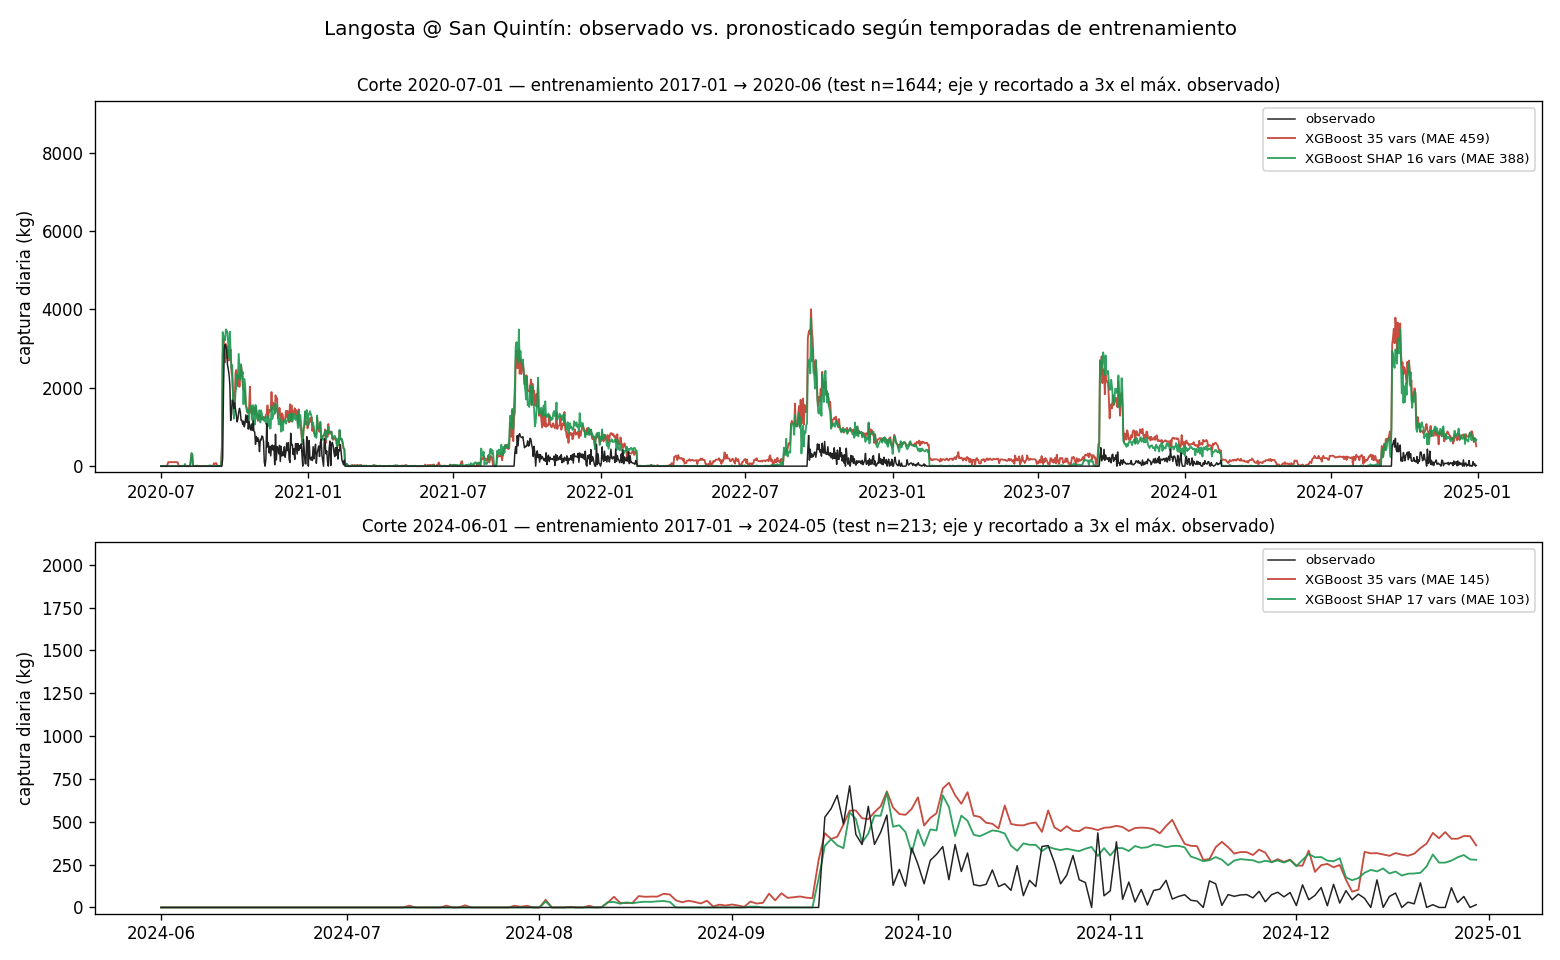
\includegraphics[width=\linewidth]{exp2_comparativa_cuts.png}
\caption{Langosta $\times$ San Quintín, observado (negro) vs. pronosticado por el XGBoost completo (35 vars, rojo) y el podado por SHAP ($\sim$16 vars, verde), en los dos cortes. Con el entrenamiento corto (arriba, hasta jun-2020) el modelo extrapola el régimen pre-bache y sobre-predice todas las temporadas post-2021; con el entrenamiento largo (abajo, hasta may-2024, con el bache incluido) sigue las temporadas recientes de captura reducida. Eje $y$ recortado a 3$\times$ el máximo observado.}
\label{fig:extension_comparativa}
\end{figure}

Cuatro lecturas se desprenden de la comparación (visibles en la Figura \ref{fig:extension_comparativa}). Primero, mover el corte de 2020 a 2024 ---es decir, meter el bache post-ola-de-calor al entrenamiento--- reduce el MAE diario a la mitad en todos los modelos \emph{tabulares} (ARIMA 331 $\to$ 178, Prophet 455 $\to$ 190, XGBoost 459 $\to$ 145, LGBM 402 $\to$ 154): al dejar de extrapolar un régimen pre-bache sobre las temporadas posteriores, los pronósticos dejan de dispararse. Es el análogo puntual del salto de cobertura de la CQR.

Segundo, el orden de los modelos se invierte. Con tres temporadas, el XGBoost con covariables (459) es \emph{peor} que ARIMA (331): 35 variables sobreajustan tan poco dato. Con siete temporadas, el mismo XGBoost (145) \emph{supera} a ambos baselines autorregresivos: las covariables de SST/MHW por fin rinden cuando hay suficientes temporadas para aprender la relación ola-de-calor $\to$ captura.

Tercero, y de forma reveladora, la poda por SHAP cambia de signo. En la fotografía previa a la unión (Tabla \ref{tab:extension_shap}) podar de 35 a 16 variables \emph{empeoraba} el modelo (MAE 424 $\to$ 445); sobre los datos unidos \emph{ayuda} en ambos cortes, y de forma marcada en el de 2024 (145 $\to$ 104, un 29\% menos de MAE). La misma regularización que era contraproducente con tres temporadas generaliza bien con siete: evidencia directa de que el sobreajuste original era un problema de \emph{volumen de datos}, no de selección de variables. El mejor modelo puntual refrescado ---XGBoost con variables seleccionadas por SHAP en el corte de 2024, MAE 103.5 y sMAPE 64.1\%--- es un salto cualitativo frente a los baselines ciegos al bache del trabajo original, y complementa a los intervalos calibrados de la CQR como entregable.

Cuarto, y es la lectura que más corrige al trabajo original: \emph{el ensamble XGBoost+LSTM ---el mejor modelo del borrador--- no sobrevive al refresco}. Con el corte de 2020 sigue encabezando la tabla (MAE 236.4 frente a 459.0 del XGBoost), pero la Figura \ref{fig:extension_comparativa_legacy} muestra que esa ventaja no viene de acertar la forma de la serie sino de \emph{amortiguarla}: con tres temporadas de entrenamiento todos los modelos extrapolan el régimen previo al bache y sobre-predicen las temporadas posteriores, y los recurrentes ---que producen una meseta suave en vez de los picos de apertura--- simplemente sobre-predicen menos. La razón entre la desviación del pronóstico y la del observado lo cuantifica: 1.58 para la LSTM y el ensamble frente a 2.37 del XGBoost, con una correlación con el observado que \emph{no} es mejor (0.61--0.67 en los cuatro modelos). Es el mismo diagnóstico que el borrador ya había anotado cualitativamente ---que el ajuste de la LSTM ``no seguía la tendencia de los datos reales'' pese a tener el menor error--- ahora medido.

Con el bache \emph{dentro} del entrenamiento el orden se invierte por completo: la LSTM pasa a MAE 499.4 y el ensamble a 561.7, ambos peores que el ARIMA (177.8) y casi cinco veces peores que el XGBoost podado por SHAP (103.5); y ahora sobre-reaccionan (razón de desviaciones 3.26 y 4.06). Es más, ambos predicen captura durante agosto, con la veda todavía abierta y semanas antes del arranque de la temporada: la LSTM aprende una rampa suave hacia el pico en lugar del salto del 15 de septiembre, y ni siquiera respeta la estructura de temporada que el calendario le da como covariable. El error en la suma de la temporada 2024-2025, la métrica que le importa a la cooperativa, es de $+626\%$ y $+704\%$ para los recurrentes frente a $+174\%$ del XGBoost. La conclusión del borrador ---que la combinación de LSTM y XGBoost era el modelo a seguir, con un error de temporada del 12.9\%--- estaba condicionada a una partición con tres temporadas y dos de prueba; con siete temporadas no se sostiene. Las $\sim$10³ observaciones por serie siguen siendo uno o dos órdenes de magnitud menos de lo que una red recurrente necesita, y el veredicto anticipa exactamente el de la prueba de techo con el TFT de la Sección \ref{sec:extension_tft}: la palanca no es la arquitectura.

\begin{figure}[htbp]
\centering
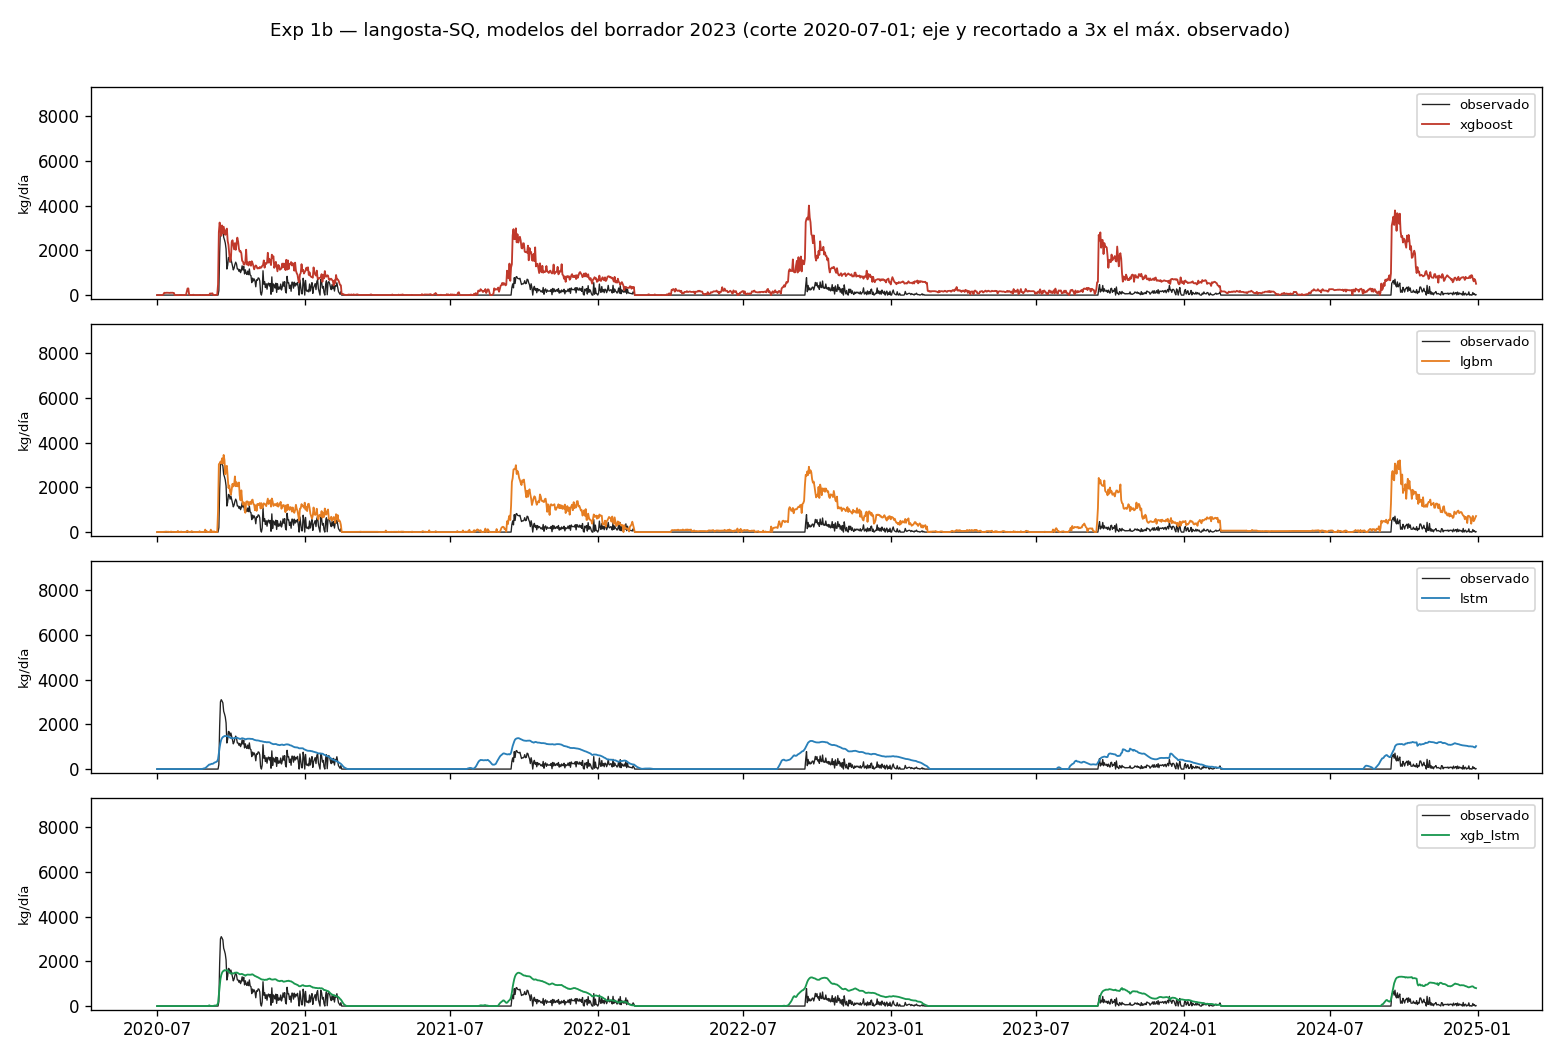
\includegraphics[width=\linewidth]{exp1_legacy_ml_2020-07-01.png}
\caption{Langosta $\times$ San Quintín en el corte 01-julio-2020: observado (negro) contra los cuatro modelos de aprendizaje del borrador. Los cuatro sobre-predicen las temporadas posteriores al bache; la LSTM y el ensamble lo hacen menos porque aplanan la serie en una meseta suave, no porque sigan mejor su forma ---de ahí su menor MAE con una correlación equivalente. Eje $y$ recortado a 3$\times$ el máximo observado.}
\label{fig:extension_comparativa_legacy}
\end{figure}

\subsection{Prueba de techo: un Transformer de fusión temporal (TFT)}
\label{sec:extension_tft}
Toda la extensión sostiene que el cuello de botella es el volumen de datos y no la sofisticación del modelo. La prueba más exigente de esa tesis es enfrentar al producto ---XGBoost con envoltura conformal--- contra una arquitectura de vanguardia y comprobar si la complejidad adicional \emph{compra} algo. Se eligió el Temporal Fusion Transformer (TFT, \citealp{lim2021}), un modelo de atención multi-horizonte con \emph{gating} de variables diseñado precisamente para series con covariables estáticas, conocidas y observadas. Se entrenó un TFT global cuantílico (\texttt{pytorch-forecasting}) sobre las 22 series especie$\times$unidad económica, con las mismas covariables de color del océano y de olas de calor marinas y la misma rejilla de 11 cuantiles de la CQR. Para una comparación de cobertura \emph{manzana con manzana} sus cuantiles se envolvieron en la \emph{misma} corrección conformal de la Sección anterior (Mondrian por serie, calibrada en temporada, en escala logarítmica), previo reordenamiento monótono por fila para eliminar el cruce de cuantiles \citep{chernozhukov2010}. Así lo que se mide es ``TFT + conformal'' frente a ``XGBoost + conformal'', en los dos cortes de prueba.

\begin{table}[htbp]
\centering
\small
\begin{tabular}{lcccccc}
\toprule
 & \multicolumn{3}{c}{Corte 2020-07-01 (bache fuera)} & \multicolumn{3}{c}{Corte 2024-06-01 (bache dentro)} \\
\cmidrule(lr){2-4}\cmidrule(lr){5-7}
Método & Cob.\ 90\% & Ancho (kg) & CRPS & Cob.\ 90\% & Ancho (kg) & CRPS \\
\midrule
TFT + conformal & 82.5\% & 2.1 & \textbf{90.6} & \textbf{91.2\%} & 1.5 & \textbf{117.8} \\
XGBoost + CQR & 97.9\% & 149.3 & 114.8 & 96.7\% & 137.8 & 130.8 \\
\bottomrule
\end{tabular}
\caption{Prueba de techo: TFT y XGBoost, ambos con la misma envoltura conformal, en los dos cortes (intervalo nominal del 90\%; cobertura empírica, ancho mediano y CRPS global). Marginalmente el TFT empata o mejora ligeramente el CRPS y, en distribución (corte 2024), queda mejor calibrado (91.2\% frente a la sobre-cobertura del 96.7\% del XGBoost); fuera de distribución (corte 2020) sub-cubre. El ancho mediano del TFT es minúsculo porque casi todos los días son fuera de temporada con captura nula.}
\label{tab:extension_tft}
\end{table}

El resultado es matizado y honesto (Tabla \ref{tab:extension_tft}). \emph{Marginalmente}, el TFT+conformal es competitivo: su CRPS global empata o supera ligeramente al del XGBoost en ambos cortes (90.6 vs.\ 114.8 en 2020; 117.8 vs.\ 130.8 en 2024), y tras el reordenamiento de cuantiles queda bien calibrado en distribución (91.2\% para el intervalo nominal del 90\% en el corte de 2024, frente a la sobre-cobertura conservadora del 96.7\% del XGBoost). El reordenamiento importó: sin él los cuantiles del TFT se cruzaban y la cobertura resultaba no-monótona. Es decir, la \emph{nitidez} probabilística cruda del Transformer no es peor que la del gradient boosting.

Lo que descalifica al TFT como producto no es su nitidez marginal sino su \emph{inestabilidad por serie}. La langosta de San Quintín ---la serie insignia--- oscila entre 40.6\% (corte 2020) y 62.0\% (corte 2024) de cobertura, con un CRPS que se dispara de 114 a 213, mientras que el XGBoost se mantiene estable (99.8\% y 96.2\%). Peor aún, en el corte de 2020 la serie de erizo de El Regasa reventó a un ancho mediano del orden de $10^{8}$ kg por desborde numérico al invertir la transformación logarítmica sobre un cuantil base mal condicionado ---un fallo que la envoltura conformal no cura porque hereda el cuantil del modelo base---. Cada corrida entrena un TFT nuevo y el ruido corrida a corrida en las series pequeñas es alto; entrenar más (8 vs.\ 30 épocas) no cambia el veredicto, la firma inconfundible de un problema limitado por \emph{datos}, no por capacidad del modelo.

El veredicto de la prueba de techo confirma la tesis de fondo. Con entre $\sim$200 y $\sim$1\,100 días de captura por serie ---uno a dos órdenes de magnitud por debajo del umbral (del orden de $10^{4}$ observaciones por grupo) donde los Transformers suelen empezar a pagar--- el TFT \emph{no supera} al XGBoost+CQR: marginalmente están en paridad, pero para una cooperativa lo que importa es una calibración \emph{estable y segura} por unidad económica, y ahí el XGBoost+CQR gana claramente por reproducibilidad y sobre-cobertura controlada. La capa conformal ---no la arquitectura--- es la que entrega la calibración. La palanca sigue siendo acumular temporadas y series, no añadir maquinaria. La justificación de diseño y esta hipótesis, enunciada \emph{antes} de correr el experimento, quedan registradas en \texttt{docs/decisions/ADR-0002-tft.md}.


\chapter{El producto operativo}
\label{cap:producto}

Un modelo que vive en un cuaderno de trabajo no le sirve a una cooperativa pesquera. Este
capítulo describe cómo se entrega el resultado del Capítulo~\ref{cap:resultados}: una
aplicación de inferencia que sirve, por especie y \ue{}, el intervalo calibrado de captura
diaria.

\section{Qué entrega y por qué así}

El producto \textbf{no es un total puntual por temporada}, y la decisión es deliberada. Como la
captura se concentra en pocos días alrededor de la apertura, la suma de las medianas diarias es
un mal estimador del total: subestima las series con picos grandes y sobreestima las de nivel
bajo. Lo que sí está calibrado ---y es lo que el sistema entrega--- es el \textbf{intervalo
diario} con su cobertura empírica verificada, más un resumen por temporada que muestra la
captura observada y la cobertura alcanzada, con la estimación central únicamente como
referencia. Es una diferencia de honestidad, no de presentación: se entrega la cantidad cuya
garantía se puede sostener.

\section{Arquitectura}

El sistema tiene tres piezas:

\begin{itemize}
  \item Una \textbf{API} (FastAPI) que, al arrancar, entrena una sola vez el modelo de
  producción ---el mismo de la Sección~\ref{sec:res_cqr}: \emph{gradient boosting} cuantílico
  en escala logarítmica con conformalización Mondrian por serie--- y deja en memoria, por serie,
  el pronóstico diario calibrado (mediana y bandas de 80 y 90\%). Los endpoints solo leen esa
  memoria, de modo que la consulta es inmediata. El entrenamiento inicial tarda entre 30 y 60
  segundos y el estado se expone en un endpoint de salud. Para despliegues reproducibles ese
  resultado puede además serializarse como \textbf{artefacto versionado}
  (\texttt{models/final/store.json}, unos 0.8 MB): es el pronóstico ya calculado ---no un
  \emph{pickle} del modelo, que ataría el despliegue a versiones exactas de las bibliotecas---
  acompañado de un manifiesto con el corte, la semilla, la versión del formato y la huella del
  conjunto de datos con el que se generó. Si el artefacto está presente la API arranca al
  instante y sirve exactamente las cifras reportadas aquí; si no, entrena en caliente y lo
  advierte en la bitácora.
  \item Un \textbf{front} estático mínimo: selector de especie y de zona, gráfico de abanico
  diario (observado contra las bandas calibradas) y un panel de \emph{backtest} por temporada
  con la captura observada y la cobertura empírica del intervalo del 90\% en temporada.
  \item Un \textbf{empaquetado} en Docker, de modo que el despliegue completo es un solo
  comando y no depende del entorno de desarrollo de quien lo corre.
\end{itemize}

El corte de prueba que define el horizonte servido es un parámetro de despliegue; por omisión se
usa 01-junio-2024, que es el corte con la calibración estable
(Sección~\ref{sec:res_moredata}). En su configuración actual sirve \textbf{28 series}: las 21 de
langosta roja más las de abulón y erizo.

\section{Lo que ve una cooperativa}

La Figura~\ref{fig:producto_api} muestra la salida de la API para tres series de langosta
elegidas por contraste, en la temporada 2024-2025.

\begin{figure}[htbp]
\centering
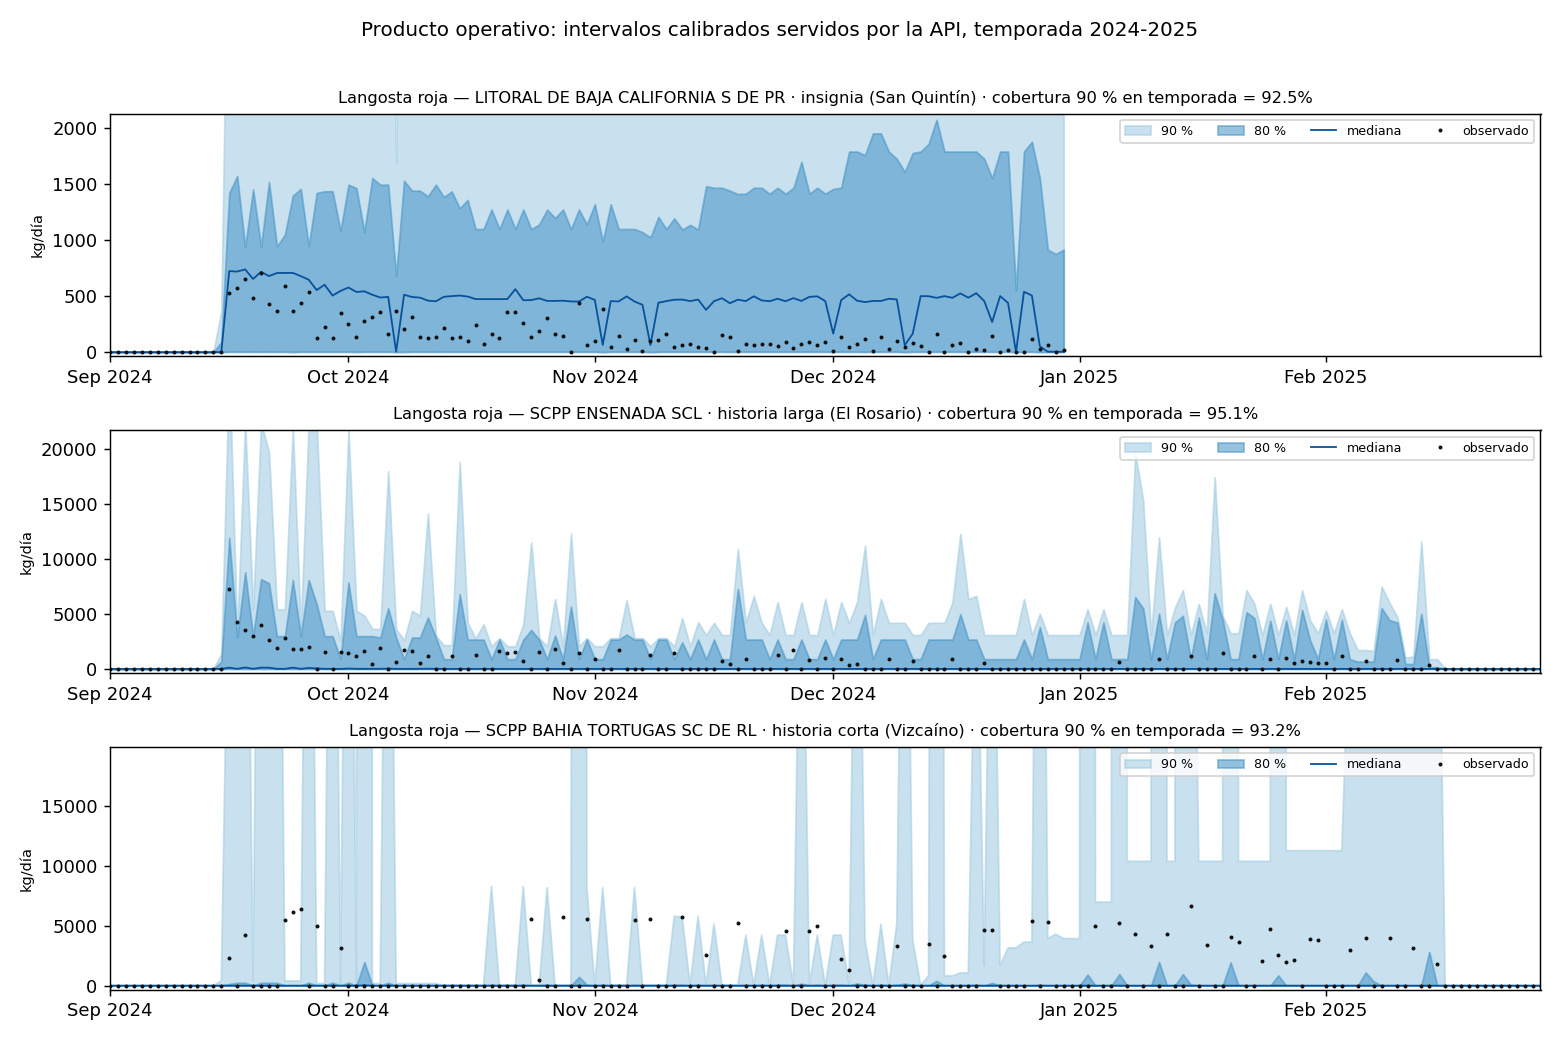
\includegraphics[width=\linewidth]{producto_api.png}
\caption{Intervalos calibrados servidos por la API para tres series de langosta roja en la
temporada 2024-2025: la serie insignia de San Quintín, una zona de historia larga (El Rosario) y
una de historia corta, incorporada solo con los avisos de CONAPESCA (Bahía Tortugas, Vizcaíno).
Los puntos son la captura observada; las bandas, los intervalos del 80 y 90\%; la línea, la
mediana. La cobertura empírica en temporada se anota en cada panel. El ancho de la banda
superior en los días de apertura es la limitación conocida del método: el cuantil alto en escala
logarítmica se amplifica al invertir la transformación.}
\label{fig:producto_api}
\end{figure}

Los tres paneles ilustran el rango de comportamiento del sistema. San Quintín, con el bache
dentro del entrenamiento, queda bien calibrada (92.5\%). El Rosario, con historia completa
2017-2026, alcanza 95.1\% y sus bandas siguen la estructura de picos de la temporada. Bahía
Tortugas, incorporada solo con avisos de CONAPESCA y con apenas dos temporadas de
entrenamiento, alcanza 93.2\% pero con bandas notoriamente más anchas: el sistema \emph{sabe}
que sabe menos de esa zona, y lo comunica ensanchando el intervalo en lugar de dar un número
falsamente preciso. Esa es exactamente la propiedad que se buscaba al reformular el pronóstico
en términos probabilísticos.

\section{Advertencias que el sistema declara}

Tres advertencias están documentadas y se muestran junto al resultado, porque un producto de
pronóstico que no declara sus límites induce confianza injustificada:

\begin{enumerate}
  \item La cobertura que reporta la interfaz es \textbf{en temporada}. Fuera de temporada la
  captura es cero y cualquier intervalo la cubre trivialmente, lo que inflaría el número.
  \item Las zonas de \textbf{historia corta} (Vizcaíno, Abreojos--La Purísima, incorporadas solo
  con datos de 2022 en adelante) están peor calibradas que las de historia larga. Su calibración
  depende de acumular temporadas, que es la conclusión de fondo de este trabajo.
  \item El sistema \textbf{no pronostica la oceanografía futura}. El horizonte llega hasta la
  última fecha con covariables disponibles: es una herramienta de pronóstico calibrado sobre el
  periodo con datos, no un oráculo de temporadas futuras arbitrarias.
\end{enumerate}

\chapter{Conclusiones}
\label{cap:conclusiones}

\section{Respuesta a las preguntas de investigación}

La evaluación de diversos modelos para predecir el volumen de capturas pesqueras en la temporada arrojó los siguientes resultados:

ARIMA, utilizado inicialmente en el contexto de todas las especies antes de ser descartado para la langosta, mostró un desempeño desfavorable y quedó fuera de la selección final.

Entre los modelos restantes, LSTM destacó como el más prometedor, exhibiendo el menor error absoluto medio y un error en la suma total de capturas de la temporada menor a los demás. Sin embargo, al visualizar los valores predichos frente a los reales, se observó que el ajuste de LSTM no seguía la tendencia de los datos reales. En contraste, XGBoost y LGBM se aproximaron mejor a dicha tendencia, a pesar de tener errores más grandes. Prophet y ARIMA, con ajustes simples que no siguen la tendencia ni se acercan a los valores reales, resultaron ininterpretables. 

El desempeño de los dos mejores modelos (LSTM y XGBoost) combinado superó a todos los demás, con un error porcentual en la suma total de pesca por temporada de 12.9\%. 

La escasez de datos de entrenamiento juega un papel importante en el mal desempeño de todos los modelos propuestos, por lo que no podemos pensar en modelos más complejos para mejorar los resultados, sino en aumentar la cantidad de datos y utilizar el mismo método para mejorar los resultados actuales.

En ese sentido, alcanzar un modelo aplicable a varias zonas de pesca y a varias especies depende de la disponibilidad de los datos para esos contextos; difícilmente los resultados de este trabajo nos acercan al resultado deseado, pero nos arrojan pistas de qué debemos hacer para alcanzarlo.

El trabajo desarrollado en esta tesis refuerza y precisa esas conclusiones iniciales. En primer lugar, la caída atípica de la temporada 2021-2022 —que el planteamiento inicial no lograba explicar y que sesgaba la evaluación de los modelos— se atribuye ahora a las olas de calor marinas de 2019-2021, un mecanismo ambiental documentado para Baja California \citep{villasenor2024} y reproducible con el índice de MHW que se incorporó al pipeline. De aquí se desprende una recomendación concreta: incluir siempre una variable de anomalía térmica de largo plazo (idealmente un índice de MHW) entre las covariables, pues es la señal que permite anticipar los años atípicos.

En segundo lugar, los experimentos con modelos multivariados y con un modelo global multi-especie confirman que el factor limitante sigue siendo la cantidad de temporadas y de series disponibles, no la sofisticación del modelo. La evidencia de transferencia positiva dentro de una misma especie entre unidades económicas es alentadora, y el enfoque jerárquico de \emph{partial pooling} que señalaba el camino a seguir quedó validado: al normalizar la variable objetivo por serie con $\log(1+y)$ —evitando que las series de mayor volumen dominen el ajuste— el modelo global pasa a ganar o empatar contra los modelos específicos en 4 de 5 series, rescatando en particular a las especies de escala pequeña. Escalar a más unidades económicas y acumular más temporadas —junto con el índice de MHW como covariable estándar y el objetivo en escala logarítmica— constituye la ruta más prometedora hacia un modelo operativo y transferible.

En tercer lugar, y como respuesta directa a esa escasez de datos, el pronóstico se reformuló en términos probabilísticos: una regresión cuantílica conformalizada sobre el modelo global entrega intervalos con cobertura cercana a la nominal y estable incluso durante las olas de calor marinas. Para una cooperativa pesquera, un rango calibrado de captura esperada es más accionable ---y más honesto--- que un único número puntual, y es el producto operativo concreto de este trabajo (Capítulo~\ref{cap:producto}).

Finalmente, la hipótesis que recorre todo el trabajo ---que el cuello de botella es el volumen de datos y no la sofisticación del modelo--- dejó de ser una conjetura y se puso a prueba. Al sumar diecinueve cooperativas de langosta (El Rosario, la costa norte, la península de Vizcaíno, el Pacífico de BCS y Bahía Magdalena, de 2 a 21 series) y desbloquear las temporadas 2022-2026 mediante la unión con los avisos de cosecha de CONAPESCA, la langosta de San Quintín ---cuya calibración ni la selección de variables por SHAP ni la optimización bayesiana de los cuantílicos habían hecho fiable--- pasó a estar bien calibrada de forma \emph{estable} (cobertura $\sim$96\%) al llevar el bache post-ola-de-calor de 2021-2022 dentro del entrenamiento, e \emph{invariante} a añadir zonas al pool; con el bache fuera del entrenamiento su cobertura era irreproducible, oscilando entre 40.6\% y 99.9\% según la composición del pool. La expansión también fijó el límite de esa transferencia: sumar zonas vecinas y de régimen térmico parecido afina el pronóstico, pero el extremo cálido del rango (Bahía Magdalena, $\sim$24$^\circ$N) ya no lo hace ---la palanca de fondo sigue siendo acumular temporadas, no zonas. Es la demostración más concreta de la tesis de fondo: la ruta hacia un modelo operativo y transferible pasa por acumular temporadas y unidades económicas ---junto con el índice de MHW como covariable estándar y el objetivo en escala logarítmica--- y no por más maquinaria estadística.

Esa hipótesis obligó también a revisar la conclusión del propio planteamiento inicial. Al re-entrenar sobre el conjunto unido los modelos que allí ganaban ---la LSTM y el ensamble XGBoost+LSTM--- su ventaja se disuelve: con tres temporadas de entrenamiento encabezan la tabla, pero por amortiguar la serie (razón de desviaciones 1.58 frente a 2.37 del XGBoost, con la misma correlación), no por seguir su forma; y con siete temporadas quedan cerca de cinco veces por detrás del XGBoost podado por SHAP, con errores de suma de temporada de $+626\%$ y $+704\%$. El error del 12.9\% que la primera iteración reportaba para el ensamble era, entonces, un artefacto de aquella partición corta y no una propiedad del modelo.

Como prueba de techo de esa afirmación se enfrentó al producto contra un Transformer de fusión temporal (TFT) con idénticas covariables y envuelto en la misma corrección conformal. El TFT resultó marginalmente algo más nítido (CRPS ligeramente a su favor en ambos cortes) pero \emph{mal calibrado}: sub-cubre en los dos cortes (70.8\% y 79.1\% para un intervalo nominal del 90\%, frente a la sobre-cobertura controlada del 96.7\% y 95.8\% del XGBoost), su diagnóstico por serie cambia de un extremo al otro al re-entrenar sobre otro pool, arrastra desbordes numéricos ocasionales y no gana nada al entrenar más épocas. Que la arquitectura de vanguardia no supere al gradient boosting con estos datos, mientras que sumar temporadas sí volvió fiable la calibración, es la confirmación más nítida de que la complejidad del modelo no es el factor limitante: lo es el volumen de datos.
% % Acknowledgements should go at the end, before appendices and references

% \acks{We would like to acknowledge support for this project
% from the National Science Foundation (NSF grant IIS-9988642)
% and the Multidisciplinary Research Program of the Department
% of Defense (MURI N00014-00-1-0637). }

% % Manual newpage inserted to improve layout of sample file - not
% % needed in general before appendices/bibliography.


\section{Limitaciones}
\label{sec:limitaciones}

Las limitaciones se enuncian en orden de gravedad para el uso del pronóstico.

\paragraph{La captura no es abundancia.} La variable objetivo es el volumen desembarcado, que
es el producto de la abundancia del recurso \emph{y} del esfuerzo pesquero: número de
embarcaciones, días efectivos de salida, precio de venta, decisiones de la cooperativa. No se
dispone de datos de esfuerzo, de modo que no es posible normalizar a captura por unidad de
esfuerzo (CPUE), que es la medida estándar en evaluación pesquera. Una parte de lo que el
modelo aprende es, por tanto, comportamiento humano y no dinámica poblacional, y una caída
puede reflejar menos salidas y no menos langosta. Esta es la limitación más importante para
interpretar los resultados en clave biológica.

\paragraph{Pocas temporadas de calibración.} Es la limitación que el propio trabajo documenta
como el cuello de botella. Con una a dos temporadas de calibración por serie, un cambio de
régimen queda fuera de la distribución aprendida: con el corte de 2020 la cobertura de la serie
insignia resulta irreproducible, oscilando según la composición del pool. El corte de 2024 es
el fiable, y lo es porque el bache está dentro del entrenamiento.

\paragraph{Zonas aproximadas por rectángulos.} La oceanografía se agrega sobre un rectángulo
costero y no sobre el polígono TURF real de cada cooperativa, que no es de acceso público. A la
resolución de los productos satelitales la aproximación es razonable, pero las cooperativas que
comparten rectángulo comparten también, por construcción, sus covariables oceanográficas.

\paragraph{Empalme de fuentes sin periodo de solape.} La unión COBI--CONAPESCA se apoya en la
continuidad del traspaso de diciembre de 2021 a enero de 2022. No existe un periodo en el que
ambas fuentes reporten simultáneamente, así que no fue posible validar exhaustivamente que las
escalas coincidan.

\paragraph{No se pronostica la oceanografía.} El horizonte útil llega hasta la última fecha con
covariables disponibles. El sistema es una herramienta de pronóstico calibrado sobre el periodo
con datos, no un oráculo de temporadas futuras arbitrarias; extenderlo exigiría alimentar
pronósticos oceanográficos, con su propia incertidumbre.

\paragraph{Dependencia de terceros.} Salvo los datos de COBI, obtenidos por convenio, las
fuentes son públicas pero externas: el trabajo depende de que Copernicus y CONAPESCA sostengan
sus procesos de publicación. Durante este trabajo, de hecho, el cliente \texttt{motuclient} de
Copernicus fue descontinuado y hubo que reescribir la ingesta.

\paragraph{Una sola especie con evidencia sólida.} Las conclusiones sobre transferencia entre
zonas están respaldadas para la langosta roja, con 21 series. Las de abulón y erizo tienen menos
series y menos temporadas, y sus resultados deben leerse como indicativos.

\section{Trabajo futuro}
\label{sec:trabajo_futuro}

\begin{enumerate}
  \item \textbf{Incorporar esfuerzo pesquero.} Es la mejora de mayor impacto científico:
  permitiría modelar CPUE y separar la señal ambiental del comportamiento de la flota. Requiere
  datos de salidas por embarcación, que las cooperativas sí registran.

  \item \textbf{Acumular temporadas.} Es la conclusión que atraviesa todo el trabajo. Cada
  temporada adicional vale más que cualquier refinamiento de modelo, y el sistema ya está
  construido para incorporarlas con un solo comando.

  \item \textbf{Conformal adaptativo por régimen.} Calibrar por separado los días con y sin ola
  de calor daría intervalos que se ensanchan automáticamente en régimen anómalo. Con una sola
  temporada de calibración por serie hoy no es robusto, pero lo será al acumular temporadas.

  \item \textbf{Polígonos TURF reales} y, con ellos, covariables oceanográficas distintas por
  cooperativa dentro de un mismo clúster.

  \item \textbf{Extender el catálogo de especies} a las que hoy tienen series cortas,
  aprovechando que el modelo global ya está diseñado para agruparlas.

  \item \textbf{Validar el producto con las cooperativas.} La utilidad real del intervalo
  calibrado solo puede evaluarse con quienes toman la decisión de compra de insumos; el
  siguiente paso natural es una temporada de uso acompañado.
\end{enumerate}


\appendix
\chapter{Gráficas de pronóstico de la primera iteración}
\label{ap:figuras}

A continuación se muestran las gráficas de valores predichos contra los valores reales en cada uno de los modelos.
\begin{figure}[htbp]
    \centering
    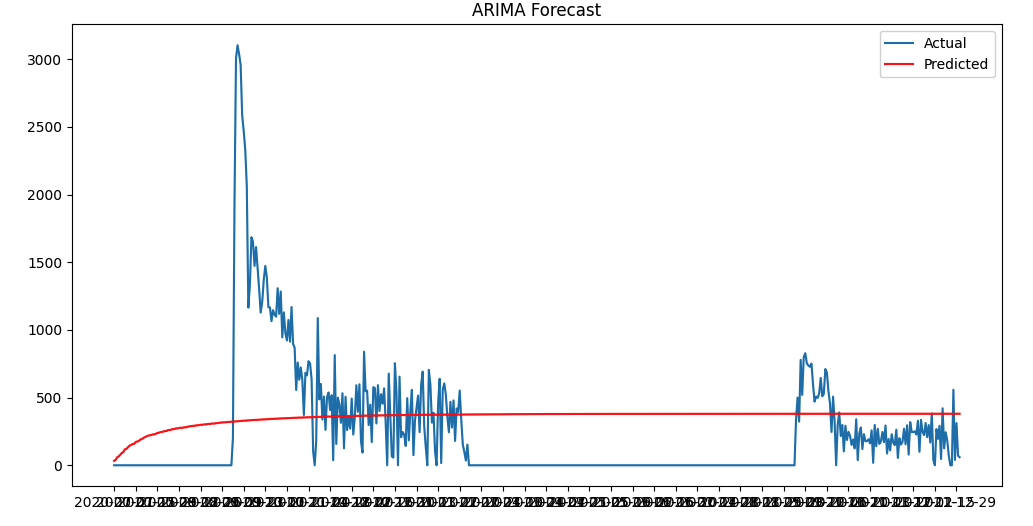
\includegraphics[width=0.9\linewidth]{arima_forecast.png}
    \caption{ARIMA: Predicción de ambas temporadas | Valores reales (azul) contra valores predichos (rojo)}
    \label{fig:pred_arima}
\end{figure}

\begin{figure}[htbp]
    \centering
    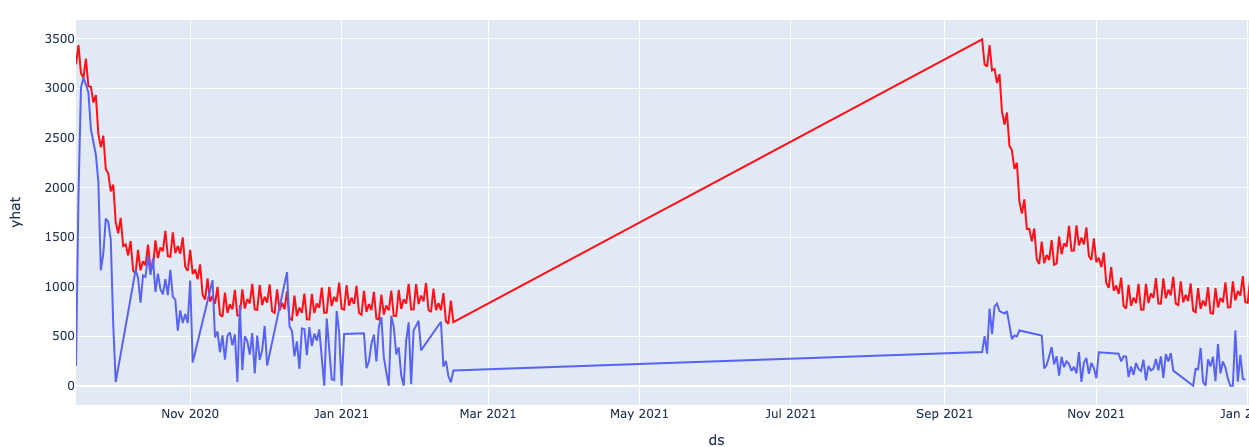
\includegraphics[width=0.9\linewidth]{prophet.png}
    \caption{Prophet: Predicción de ambas temporadas | Valores reales (azul) contra valores predichos (rojo)}
    \label{fig:pred_prophet}
\end{figure}
\begin{figure}[htbp]
    \centering
    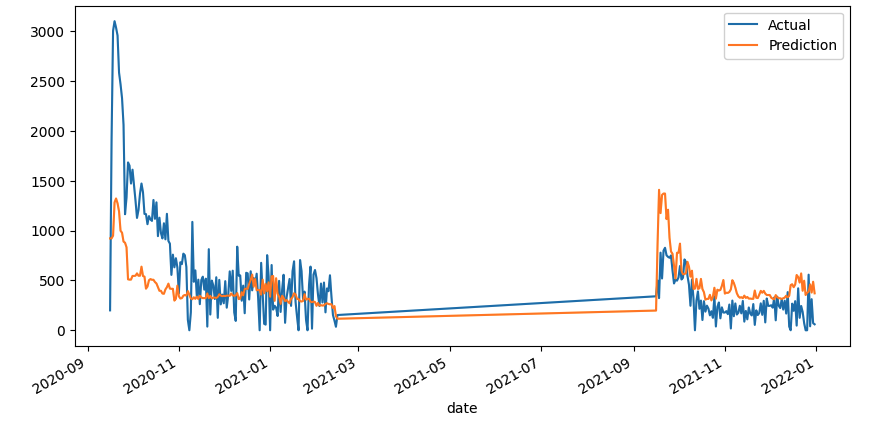
\includegraphics[width=0.9\linewidth]{xgboost_final.png}
    \caption{XGBoost: Predicción de ambas temporadas | Valores reales (azul) contra valores predichos (naranja)}
    \label{fig:pred_xgboost}
\end{figure}

\begin{figure}[htbp]
    \centering
    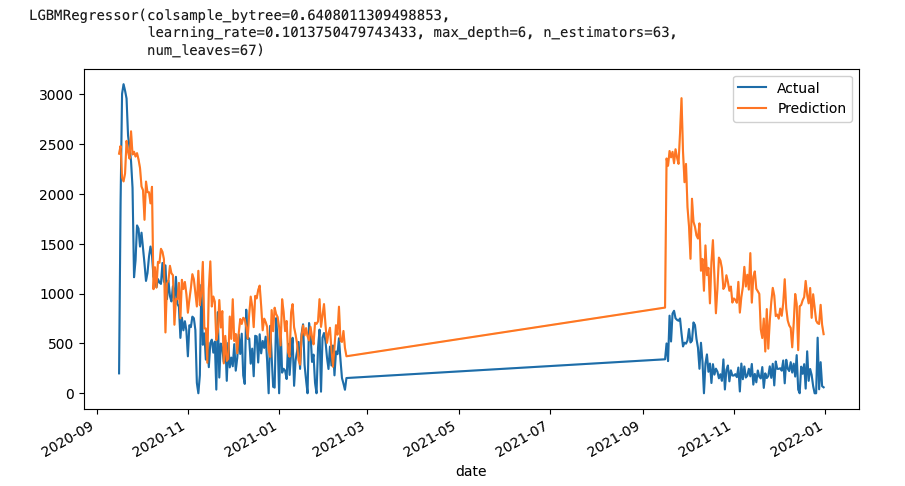
\includegraphics[width=0.9\linewidth]{lgbm_final.png}
    \caption{LGBM:  Predicción de ambas temporadas | Valores reales (azul) contra valores predichos (naranja)}
    \label{fig:pred_lgbm}
\end{figure}

\begin{figure}[htbp]
    \centering
    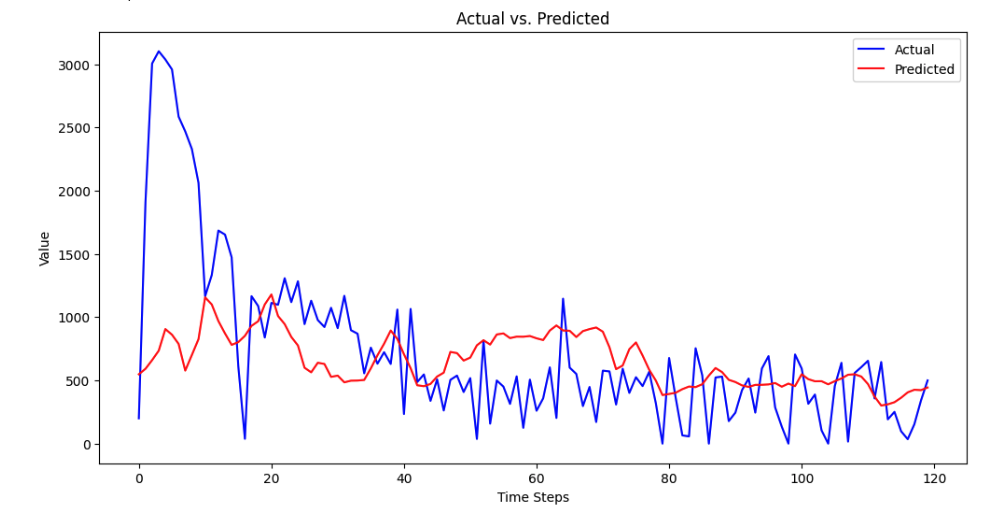
\includegraphics[width=0.9\linewidth]{final_first_season.png}
    \caption{XGBoost + LSTM | Predicción temporada 2020-2021: Valores reales (azul) contra valores predichos (rojo)}
    \label{fig:pred_ensemble_2020}
\end{figure}

\begin{figure}[htbp]
    \centering
    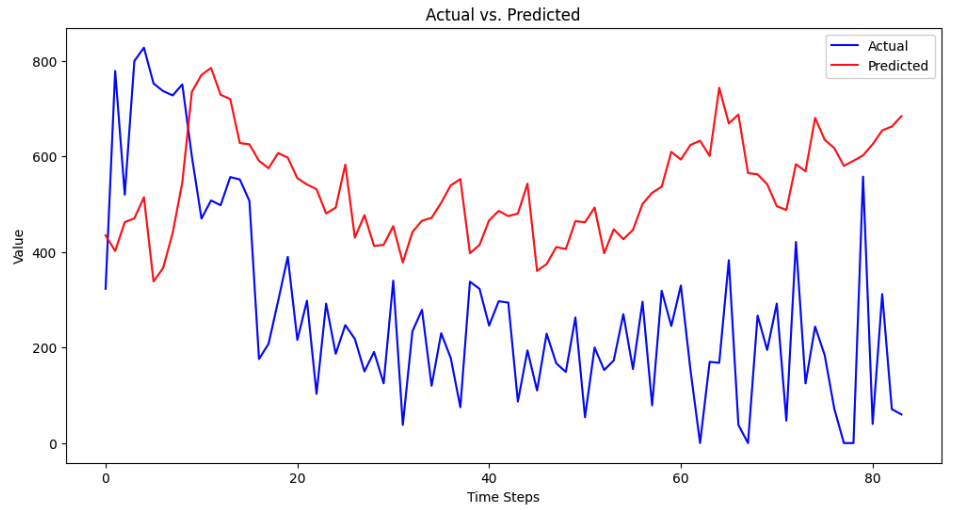
\includegraphics[width=0.9\linewidth]{image.png}
    \caption{XGBoost + LSTM | Predicción temporada 2021-2022: Valores reales (azul) contra valores predichos (rojo)}
    \label{fig:pred_ensemble_2021}
\end{figure}

\begin{figure}[htbp]
    \centering
    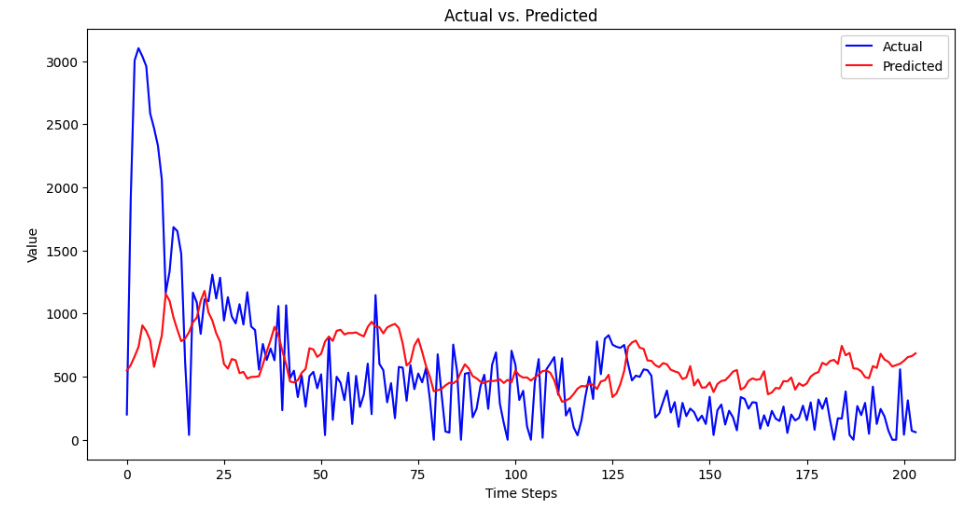
\includegraphics[width=0.9\linewidth]{final_two_seasons.png}
    \caption{XGBoost + LSTM | Predicción temporadas 2020-2021 y 2021-2022: Valores reales (azul) contra valores predichos (rojo). Nota: Aquí no aparecen las fechas consideradas como veda (periodo entre temporadas)}
    \label{fig:pred_ensemble_ambas}
\end{figure}


\vskip 0.2in


\chapter{Descripción de las variables}
\label{ap:variables}

\subsection{Descripción de los datos}
El conjunto de datos utilizado está compuesto de fecha 'ds', variable objetivo 'y' y 16 variables regresoras 'xi', como se muestra en la tabla 4.
\begin{table}[htbp]
\centering
\caption{Muestra de conjunto de datos}
\label{tab:datos}
\begin{tabular}{cccccccccccccccccc}
\toprule
ds & y & x1 & x2 & x3 & ... & x16 \\
\midrule
15/12/17 & 500 & 0.1556 & 0.2067 & 17.6501 & ... & 11.3717 \\
16/12/17 & 598 & 0.2126 & 0.2732 & 12.5639 &  ... & 10.0574 \\
17/12/17 & 1018 & 0.0677 & 0.1281 & 22.6158 & ... & 14.8350 \\
18/12/17 & 0 & 0.0520 & 0.0985 & 7.8426 & ... & 12.2488 \\
19/12/17 & 1568 & 0.0726 & 0.1186 & 9.8166 & ... & 11.8934 \\
19/12/17 & 1568 & 0.0726 & 0.1186 & 9.8166 & ... & 11.8934 \\
... & ... & ... & ... & ... & ... & ... \\
31/12/21 & 60 & 0.0648	& 0.1079 & 99.7545 & ... &	12.0536 \\
\bottomrule
\end{tabular}
\end{table}

A continuación se describe cada una de las variables:
\begin{itemize}
    \item \textbf{Variable ds | Fecha:} El conjunto de datos cuenta con observaciones diarias desde el 01 de enero de 2017 hasta el 31 de diciembre de 2022. La fecha tiene el formato d-m-y
    \item \textbf{Variable y | Volumen total de pesca:} Es la variable objetivo. Se trata del volumen total de pesca para la fecha dada; el valor es flotante y representa kilogramos.
       \item \textbf{Variable x1 | Aerosol Optical Thickness over Water:}
    Medida de la cantidad de aerosoles en la atmósfera sobre cuerpos de agua.

    \item \textbf{Variable x2 | Aerosol Optical Thickness over Water+Land:}
    Similar a la anterior, pero considera tanto agua como tierra en la medición de aerosoles atmosféricos.

    \item \textbf{Variable x3 | Cloud Fraction:}
    Fracción del cielo cubierta por nubes, expresada como un valor entre 0 y 1.

    \item \textbf{Variable x4 | Depth of the Bottom of the Euphotic Layer:}
    Profundidad a la que la luz del sol es suficiente para la fotosíntesis en el océano.

    \item \textbf{Variable x5 | Secchi Disk Depth:}
    Profundidad a la que un disco blanco (Secchi) es visible en el agua y se utiliza para medir la transparencia del agua.

    \item \textbf{Variable x6 | Heated Layer Depth:}
    Profundidad de la capa calentada en el agua, que puede afectar las propiedades térmicas.

    \item \textbf{Variable x7 | Particulate Backscattering Coefficient:}
    Medida de la cantidad de luz dispersada por partículas en el agua en dirección opuesta a la fuente de luz.

    \item \textbf{Variable x8 | Coloured Dissolved Detrital Organic Materials Absorption Coefficient:}
    Coeficiente de absorción de materiales orgánicos disueltos y detritales que dan color al agua.

    \item \textbf{Variable x9 | Diffuse Attenuation Coefficient:}
    Tasa de disminución de la luz a medida que se propaga a través del agua debido a la dispersión y absorción.

    \item \textbf{Variable x10 | Relative Excess of Radiance:}
    Diferencia entre la radiación observada y la radiación esperada en un entorno dado.

    \item \textbf{Variable x11 | Normalised Remote Sensing Reflectance:}
    Reflectancia normalizada utilizada en teledetección para caracterizar la cantidad de luz reflejada por una superficie.

    \item \textbf{Variable x12 | Normalised Fluorescence Line Height:}
    Altura normalizada de la línea de fluorescencia, que puede indicar la actividad biológica en el agua.

    \item \textbf{Variable x13 | Particulate Organic Carbon:}
    Concentración de carbono orgánico en partículas suspendidas en el agua.

    \item \textbf{Variable x14 | Particulate Inorganic Carbon:}
    Concentración de carbono inorgánico en partículas suspendidas en el agua.

    \item \textbf{Variable x15 | Inorganic Suspended Particulate Matter Concentration:}
    Concentración de materia particulada inorgánica suspendida en el agua.

    \item \textbf{Variable x16 | Photosynthetically Available Radiation:}
    Radiación disponible para la fotosíntesis, es decir, la cantidad de luz que puede ser utilizada por los organismos fotosintéticos.
\end{itemize}

En el documento de GlobColour \cite{globcolour2020}, se proporciona información detallada sobre el procesamiento de cada variable.



\cleardoublepage
\addcontentsline{toc}{chapter}{Referencias}
\bibliographystyle{plainnat}
\bibliography{referencias}

\end{document}
